\documentclass[
twocolumn,
pra,showpacs,preprintnumbers,amsmath,amssymb]{revtex4}

\usepackage{times}
\usepackage{graphicx}
\usepackage{amssymb}
\usepackage{amsthm}
\usepackage{amsmath}
\usepackage{dsfont}
\usepackage{bm}
\usepackage{mathrsfs}
\usepackage{bbold}


\begin{document}

\title{Theory of Maxwell's fish eye with mutually interacting sources and drains}
\author{Ulf Leonhardt$^1$ and Sahar Sahebdivan$^{2,3}$}
\affiliation{
\normalsize{
$^1$Department of Physics of Complex Systems,
Weizmann Institute of Science, Rehovot 761001, Israel\\
$^2$Quantum Optics, Quantum Nanophysics, Quantum Information,
University of Vienna, Boltzmanngasse 5, A-1090 Vienna, Austria\\
$^3$School of Physics and Astronomy, University of St Andrews,
North Haugh, St Andrews KY16 9SS, UK}
}
\date{\today}

\begin{abstract}
Maxwell's fish eye is predicted to image with a resolution not limited by the wavelength of light. However, interactions between sources and drains may ruin the subwavelength imaging capabilities of this and similar absolute optical instruments. Nevertheless, as we show in this paper, at resonance frequencies of the device, an array of drains may resolve a single source or, alternatively, a single drain may scan an array of sources, no matter how narrowly spaced they are. It seems that near-field information can be obtained from far-field distances. 
\end{abstract}

\pacs{68.37.-d, 42.25.Bs}

\maketitle

\section{Introduction}

Attempts to overcome or circumvent Abbe's diffraction limit of optical imaging \cite{Abbe,BornWolf}, the limit of about half the wavelength in optical resolution, have traditionally been greeted with controversy \cite{RMP}. Controversy arises, partly because neither imaging nor resolution are unambiguously defined terms, partly because of the long history of ways around the resolution limit \cite{History}. Perfect lensing with negative refraction \cite{Pendry} was no exception \cite{Perfectdebate} and neither was perfect imaging \cite{Fish,Fish3D} with absolute optical instruments \cite{BornWolf,Maxwell,Synge}. In the latter, the controversy \cite{TycZhang,Blaikie1,Leo1,Merlin1,LPre,Sailing1,Sailing2,Kinsler1,LeoSahar,Merlin2,Kinsler2,Leo2,Blaikie2,MinanoSim,Hao,Pazynin,TycDanner,Sailing3} focused on the role of detection --- a perfect image only appears when it is detected. 

In this paper, we focus on absolute optical instruments \cite{BornWolf,Maxwell,Synge} with positive refraction and investigate the role of interacting sources and detectors in perfect imaging. Our paper generalises the simple, one--dimensional model \cite{1D} that has already explained the data of the experiment \cite{Minano} and draws further conclusions: we establish limitations and prospects that arise from interactions and resonances (Fig.~\ref{title}). Those factors are fundamentally decisive even before practical matters such as losses in the device \cite{Nieto} and noise and uncertainty in the data \cite{NietoBook} are taken into account. 
%%%
\begin{figure}[t]
\begin{center}
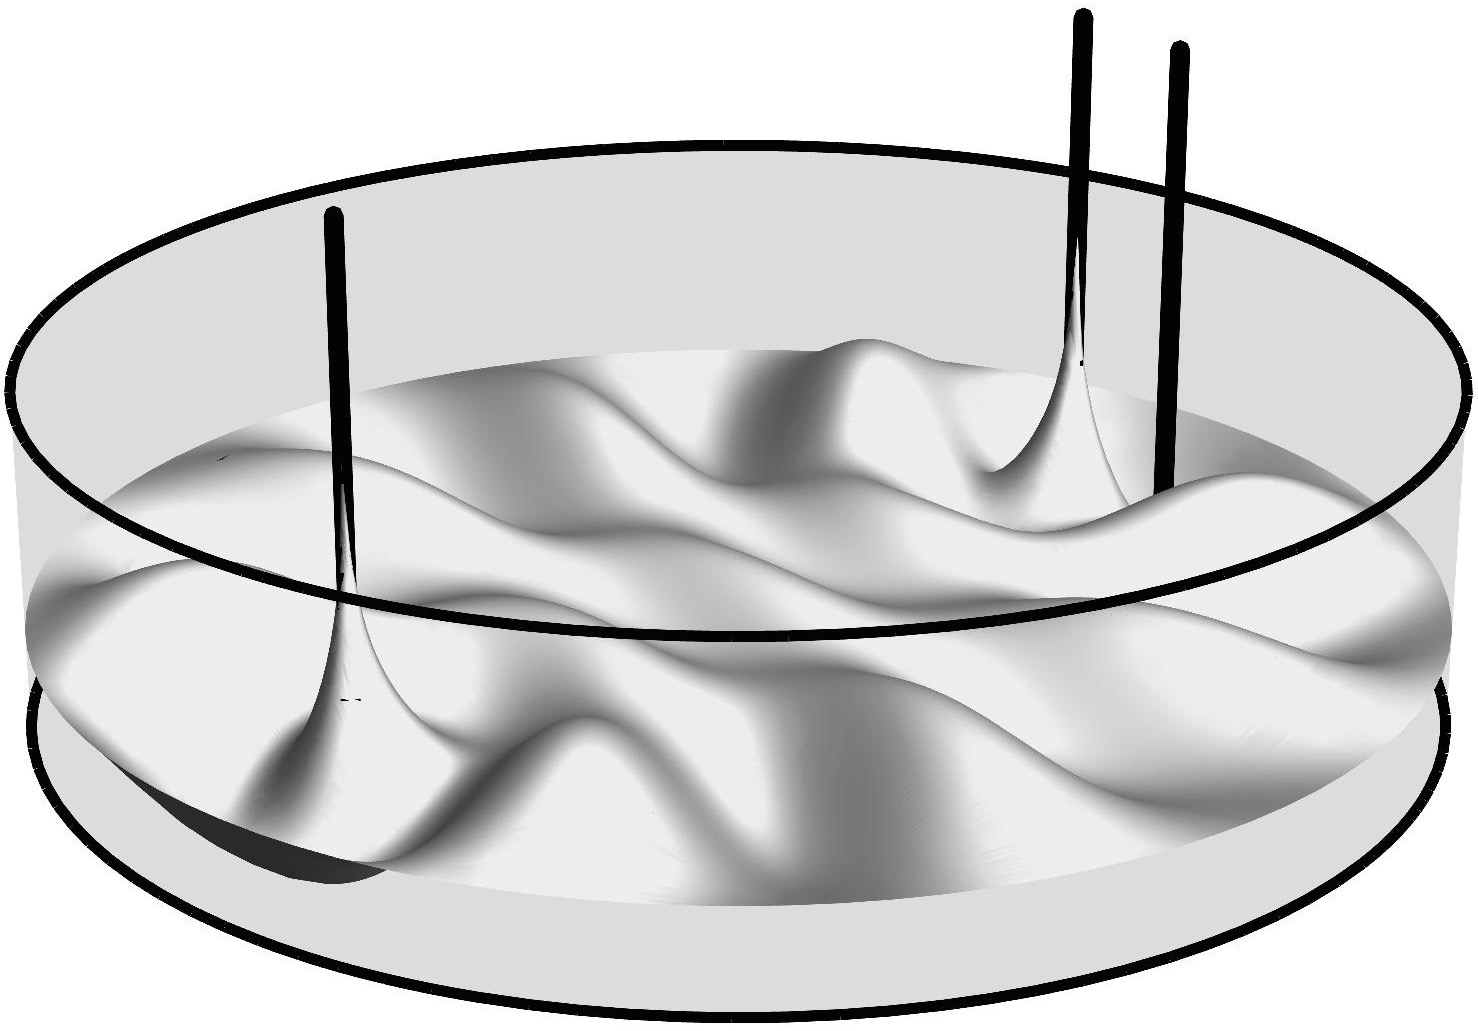
\includegraphics[width=19.5pc]{fig1.jpg}
\caption{
\small{
Scheme: absolute optical instrument with mutually interacting sources and drains. Radiation enters and leaves the device via cables that act as sources and drains. The instrument shown is Maxwell's fish eye \cite{Maxwell} surrounded by a mirror \cite{Fish} with radiation at resonance. In the figure one source faces two drains. Only the drain opposite to the source couples the radiation out, the other does not transmit. In this case the two drains resolve the position of the source. The roles of sources and drains may be reversed: the figure may also represent two sources scanned by one movable drain. Only when the drain is at the image position of one of the sources it transmits, even if the sources were much closer than the wavelength. Note that the imaging/scanning regimes work only near resonances.
}
\label{title}}
\end{center}
\end{figure}
%%%

The crucial role of detection becomes clear in Feynman's argument \cite{Feynman,Quabis,Carminati} against the diffraction limit \cite{Abbe,BornWolf}: as Maxwell's electromagnetism is invariant upon time reversal, the electromagnetic wave emitted from a point source may be reversed and focused into a point with point--like precision, not limited by diffraction \cite{Abbe,BornWolf}. However, for this the entire emission process must be reversed, including the source: in place of the point source, a point drain must sit at the focal position \cite{Quabis,Carminati}. The time--reversed source, the drain, is the detector taking the image of the source. Without getting absorbed at the detector, the focused wave will rebound, the superposition of the focusing and the expanding, rebounding wave will produce a diffraction--limited spot \cite{Quabis,Carminati}.

Experiments with microwaves \cite{deRosny} have confirmed the role of detection in perfect focusing. Here the emitted radiation was actively time--reversed, upon which it focused at the point of emission where the time reverse of the source current localised it with a precision much better than the diffraction limit \cite{Abbe,BornWolf}. Absolute optical instruments \cite{BornWolf,Maxwell,Synge} may perform the time reversal of the field with perfectly passive materials and send the reversed wave to a different spatial position than the source. As in the case of the microwave experiments \cite{deRosny}, a detector is required to sharpen the image, but this detector may be as passive as the device. Absolute optical instruments \cite{BornWolf,Maxwell,Synge} may thus perform passive perfect imaging \cite{Fish}.

Two sets \cite{Ma,Minano} of microwave experiments appeared to have confirmed the idea \cite{Fish} of perfect imaging with absolute optical instruments \cite{BornWolf,Maxwell,Synge}. The first experiment \cite{Ma} clearly demonstrated the need and the effect of a detector at the focus of the radiation emitted from a single source. In the second set of experiments \cite{Minano}, the detector was movable. Close to the resonance frequencies of the absolute optical instrument the detector did only record the field when moved close to the correct imaging position, much closer than the diffraction limit \cite{Abbe,BornWolf}. The movable detector could scan the single source from a far--field distance. In the first set of experiments \cite{Ma}, the radiation of two sources was also sent to an array of detectors that appeared to have resolved them when they were significantly closer than the wavelength. However, doubts about the validity of the published data have been cast \cite{EoC} and later confirmed \cite{Sailing3}.

Perfect imaging with absolute optical instruments \cite{Fish,Fish3D} seems therefore restricted by some qualifications: so far it has only worked for a single--source single--drain configuration and near the resonance frequencies of the device. On the other hand, Feynman's argument appears to be universally valid. What was the problem? In the experiments \cite{Ma,Minano} the sources and drains are interacting with each other. They are cables coupling in and out microwave radiation to and from the device (Fig.~\ref{title}). They establish an equilibrium of radiation that depends on their transmission and reflection coefficients. In Feynman's argument, however, the detector ceases to operate when the field is detected, and the drain definitely does not act on the source --- the future does not act back to the past. 

In this paper, we investigate what mutually interacting detectors can do nevertheless. As we are going to show, an array of detectors can image a point source with arbitrary precision and a single detector can scan an array of near--field sources from a far--field distance with perfect fidelity. However, for this the radiation has to be at resonance and the number of detectors or sources must not exceed the number of waves (in a sense we will make precise).

Our analysis becomes possible thanks to a theoretical model for mutually interacting sources and drains we develop in this paper. Modelling such sources and drains analytically has been a major challenge \cite{Kinsler1,TycDanner,Gonzales,Xu,MaOng}, full numerical simulations \cite{MinanoSim,Hao} have been difficult due to the large difference in the scales involved (the field localization near the sources and drains versus the wave propagation in the device). Our analytic theory draws from a simple, one--dimensional model \cite{1D} that has explained the experimental data \cite{Minano}. Inspired by the Lagrangian of the electromagnetic field interacting with a current \cite{LL2}, we construct a Lagrangian that reproduces the one--dimensional model \cite{1D} and has the advantage of being extendable to higher dimensions --- in our case two --- where imaging takes place. Our Lagrangian theory represents a device--independent, idealized model beyond numerical simulations. 

\section{Model}

\subsection{Lagrangian}

Consider the electromagnetic field in both the device and the cables that act as the input and output channels (Fig.~\ref{title}). The field shall be polarized such that only one component $A$ of the vector potential is relevant. We describe the field dynamics by the Lagrangian density 
%%%%%%
\begin{equation}
\mathscr{L} = \mathscr{L}_0 + \sum_m \mathscr{L}_m
\end{equation}
%%%%%%
that consists of the Lagrangian density $\mathscr{L}_0$ of the field inside the device, 
%%%%%%
\begin{equation}
\mathscr{L}_0 = \frac{1}{2} \left( n^2 \left(\partial_t A\right)^2 - \left(\nabla A\right)^2\right) ,
\end{equation}
%%%%%%
and the Lagrangian densities $\mathscr{L}_m$ of the field in the cables and their interaction at their ports of entrance to the device:
%%%%%%
\begin{equation}
\mathscr{L}_m = \frac{1}{2} \left(\left(\partial_t A\right)^2 - \left(\partial_m A\right)^2\right) 
-g A \left(\partial_m A\right) \delta (z-z_m) \,.
\label{cablelagrangian}
\end{equation}
%%%%%%
Here $n$ denotes the refractive--index profile in the device. The archetype of the absolute optical instrument \cite{BornWolf} is Maxwell's fish eye \cite{Maxwell,Dover} with the profile
%%%%%%
\begin{equation}
n = \frac{2}{1+|z|^2} \,.
\label{maxwell}
\end{equation}
%%%%%%
We consider wave propagation in two--dimensional space described by the complex coordinate $z=x+iy$ on the Cartesian $(x,y)$ plane (Fig.~\ref{title}). The wave propagation with refractive--index profile (\ref{maxwell}) is equivalent \cite{Dover} to the free wave propagation on the unit sphere $(X,Y,Z) = (\sin\theta\cos\phi, \sin\theta\sin\phi, \cos\theta)$. Both are related to each other by stereographic projection (Fig.~\ref{figstereo}):
%%%%%%
\begin{equation}
z = \frac{X+iY}{1-Z} = e^{i\phi}\cot\frac{\theta}{2}\,.
\label{stereo}
\end{equation}
%%%%%%
%%%
\begin{figure}[h]
\begin{center}
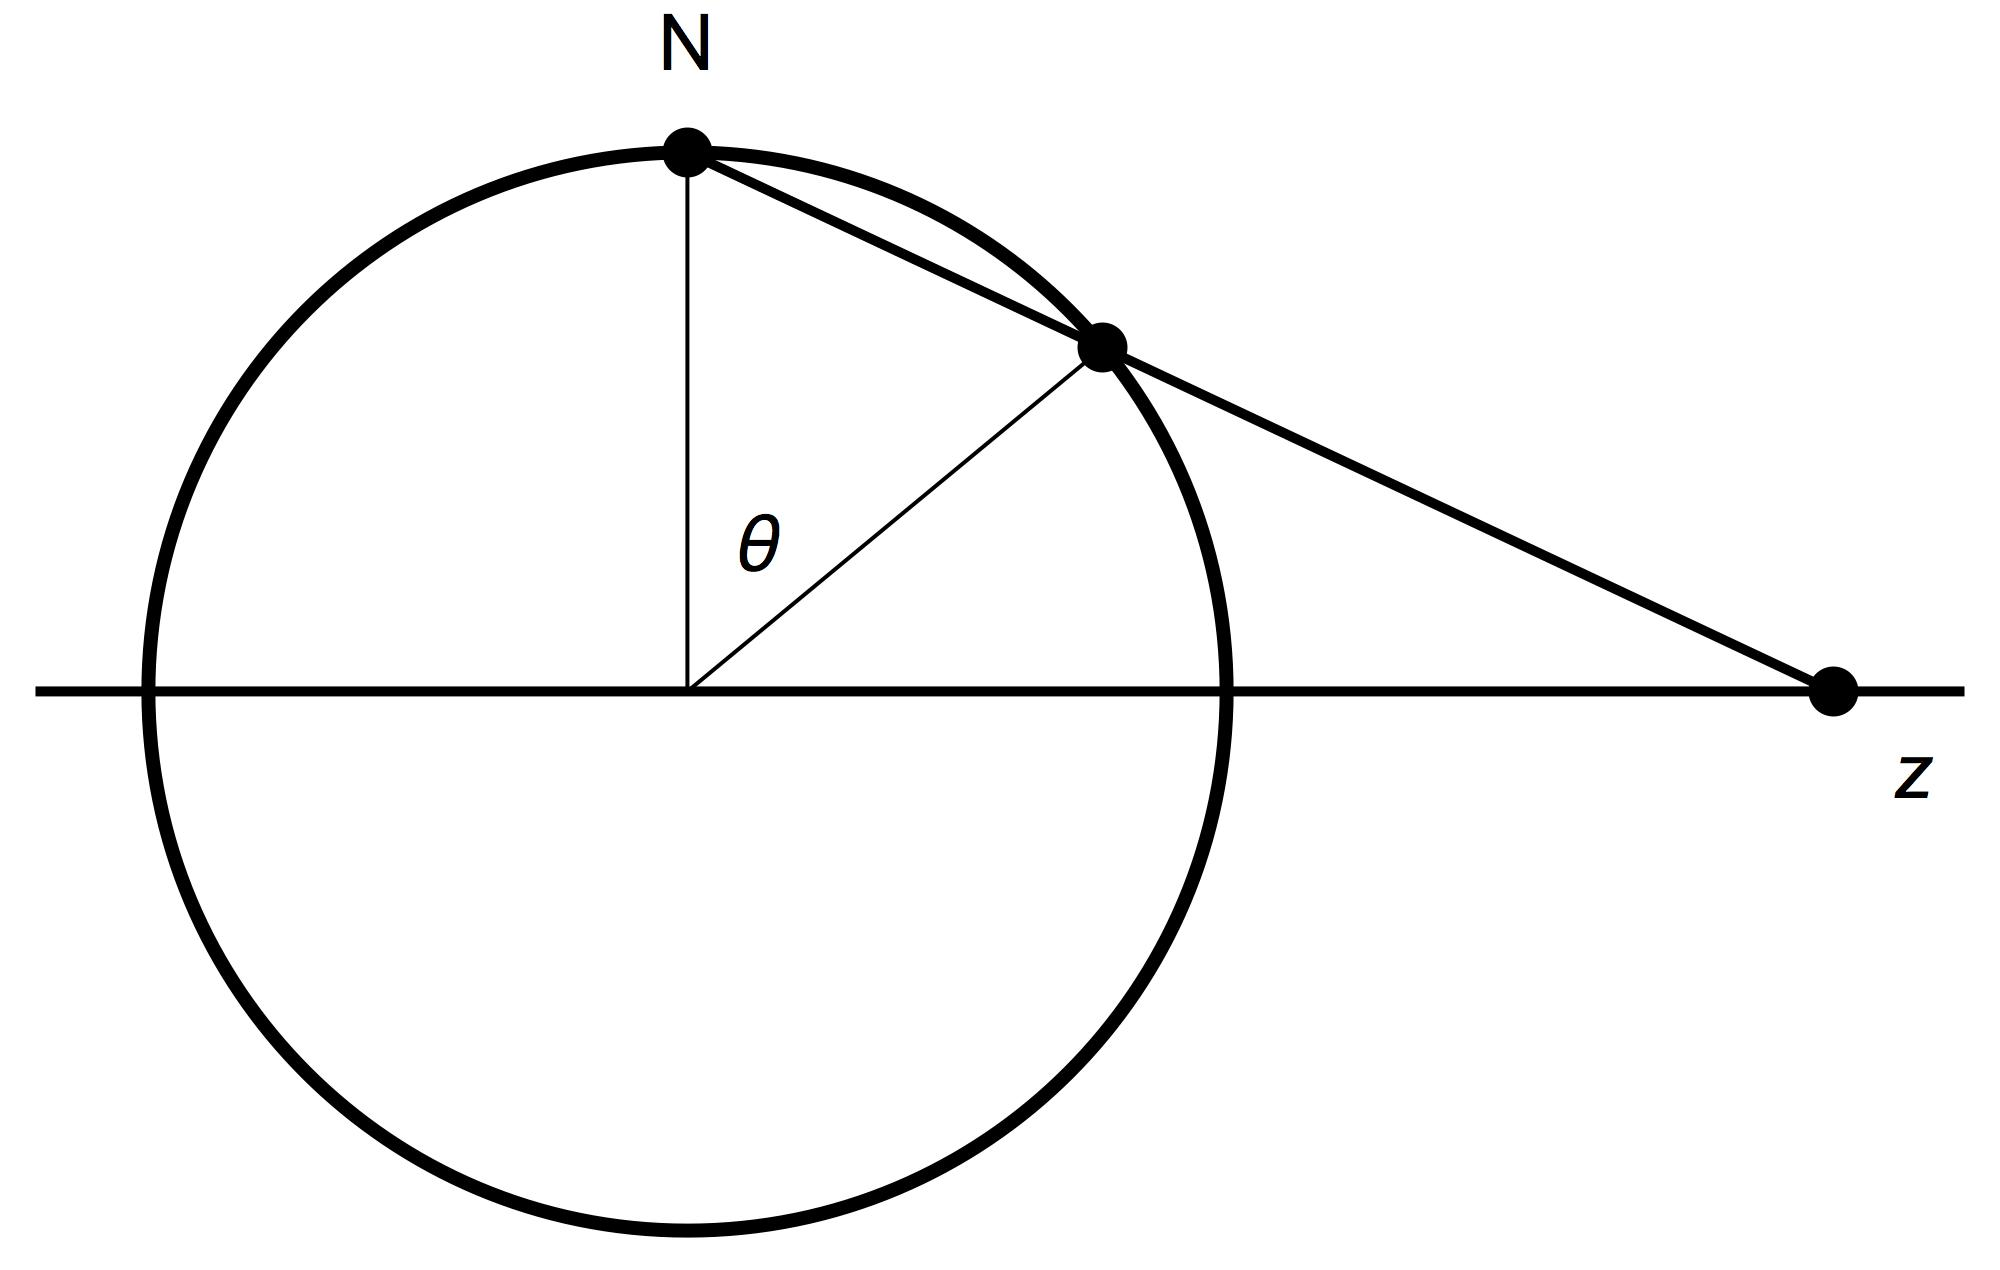
\includegraphics[width=20.0pc]{fig2.jpg}
\caption{
\small{
Stereographic projection. The plane of Maxwell's fish eye is the stereographic projection of the surface of the sphere (shown in a cut). Experiments \cite{Ma} in the $z$--plane with the refractive index profile of Eq.~(\ref{maxwell}) are equivalent to experiments  \cite{Minano} on the sphere with $n=1$.
}
\label{figstereo}}
\end{center}
\end{figure}
%%%

In the language of transformation optics \cite{Dover} the unit sphere represents the virtual and the plane with the profile of Eq.~(\ref{maxwell}) the physical space. We shall mentally switch between the two pictures whenever one is more convenient than the other. As unit of length we take the radius of the device and as time unit the round--trip time divided by $2\pi$. 

In the model of the field in the cables, Eq.\ (\ref{cablelagrangian}), we assume that the same field $A$ as in the inside of the device extends to the cables. The cables are idealized to be one--dimensional; the propagation coordinate along the $m$-th cable we denote by $s_m$, the derivative with respect to $s_m$ by $\partial_m$; the port of entrance we put at $s_m=0$. For the interaction term $g A \left(\partial_m A\right) \delta (z-z_m)$ we have assumed that the flux of the field in the cable, $\partial_mA$, generates with coupling strength $g$ a current $j$ localized at the port of entrance. The current interacts with the field according to the standard electromagnetic coupling $jA$ in the Lagrangian density \cite{LL2}. In short, we have assumed the cables act as point antennas.

\subsection{Field equations}

Having established the Lagrangian, we obtain the field equations from the Euler--Lagrange equation \cite{LL2}. We separate them into the field equation inside the device and the equation in the cables, and get
%%%%%%
\begin{eqnarray}
\left(n^2\partial_t^2 - \nabla^2\right) A &=& -g\sum_m\left(\partial_m A\right)\delta(z-z_m) \,,
\label{eq1} \\
\left(\partial_t^2 - \partial_m^2\right) A &=& g A(z_m)\, \partial_m \delta(s_m) \,.
\label{eq2}
\end{eqnarray}
%%%%%%
For the field equation in the cables we have read $\delta(z-z_m)$ from the perspective of the cables, {\it i.e.}\ as $\delta(s_m)$. We consider an equilibrium of the radiation in the device and the cables, and so we write $A$ as a monochromatic field oscillating with circular frequency $k$ (that, thanks to our choice of units, agrees with the free--space wavenumber). Furthermore, we decompose the field into a stationary component $\Psi$ localized in the device and the components $\chi_m$ localized in the cables:
%%%%%%
\begin{equation}
A = \big(\Psi + \sum_m \chi_m\big) e^{-ikt} \,.
\end{equation}
%%%%%%
We obtain from Eqs.~(\ref{eq1}) and (\ref{eq2}) the stationary wave equations
%%%%%%
\begin{eqnarray}
\left(\nabla^2 + n^2k^2\right) \Psi &=& g\sum_m\left(\partial_m \chi_m\right)\delta(z-z_m) \,,
\label{w1} \\
\left(\partial_m^2 + k^2 \right) \chi_m &=& - g \Psi(z_m)\, \partial_m \delta(s_m) \,.
\label{w2}
\end{eqnarray}
%%%%%%
From Eq.~(\ref{w2}) follows that $\chi_m$ jumps by $-g\Psi(z_m)$ at $s_m=0$. After the jump $\chi_m$ is zero, because the $\chi_m$-components of the field are required to be localized in the cables. Consequently, the field at the end of each cable must be equal to $g$ times the field in the device:
%%%%%%
\begin{equation}
\chi_m(0)=g \Psi(z_m) \,.
\label{fields}
\end{equation}
%%%%%%
In the cables we have the oscillatory solutions
%%%%%%
\begin{equation}
\chi_m = a_m e^{iks_m} + a_m' e^{-iks_m} \,.
\label{chi}
\end{equation}
%%%%%%
The coefficients $a_m$ describe the incoming amplitudes, the coefficients $a_m'$ the outgoing amplitudes. For a drain representing a detector the incoming amplitude $a_m$ is zero (Fig.~\ref{figscattering}).
%%%
\begin{figure}[h]
\begin{center}
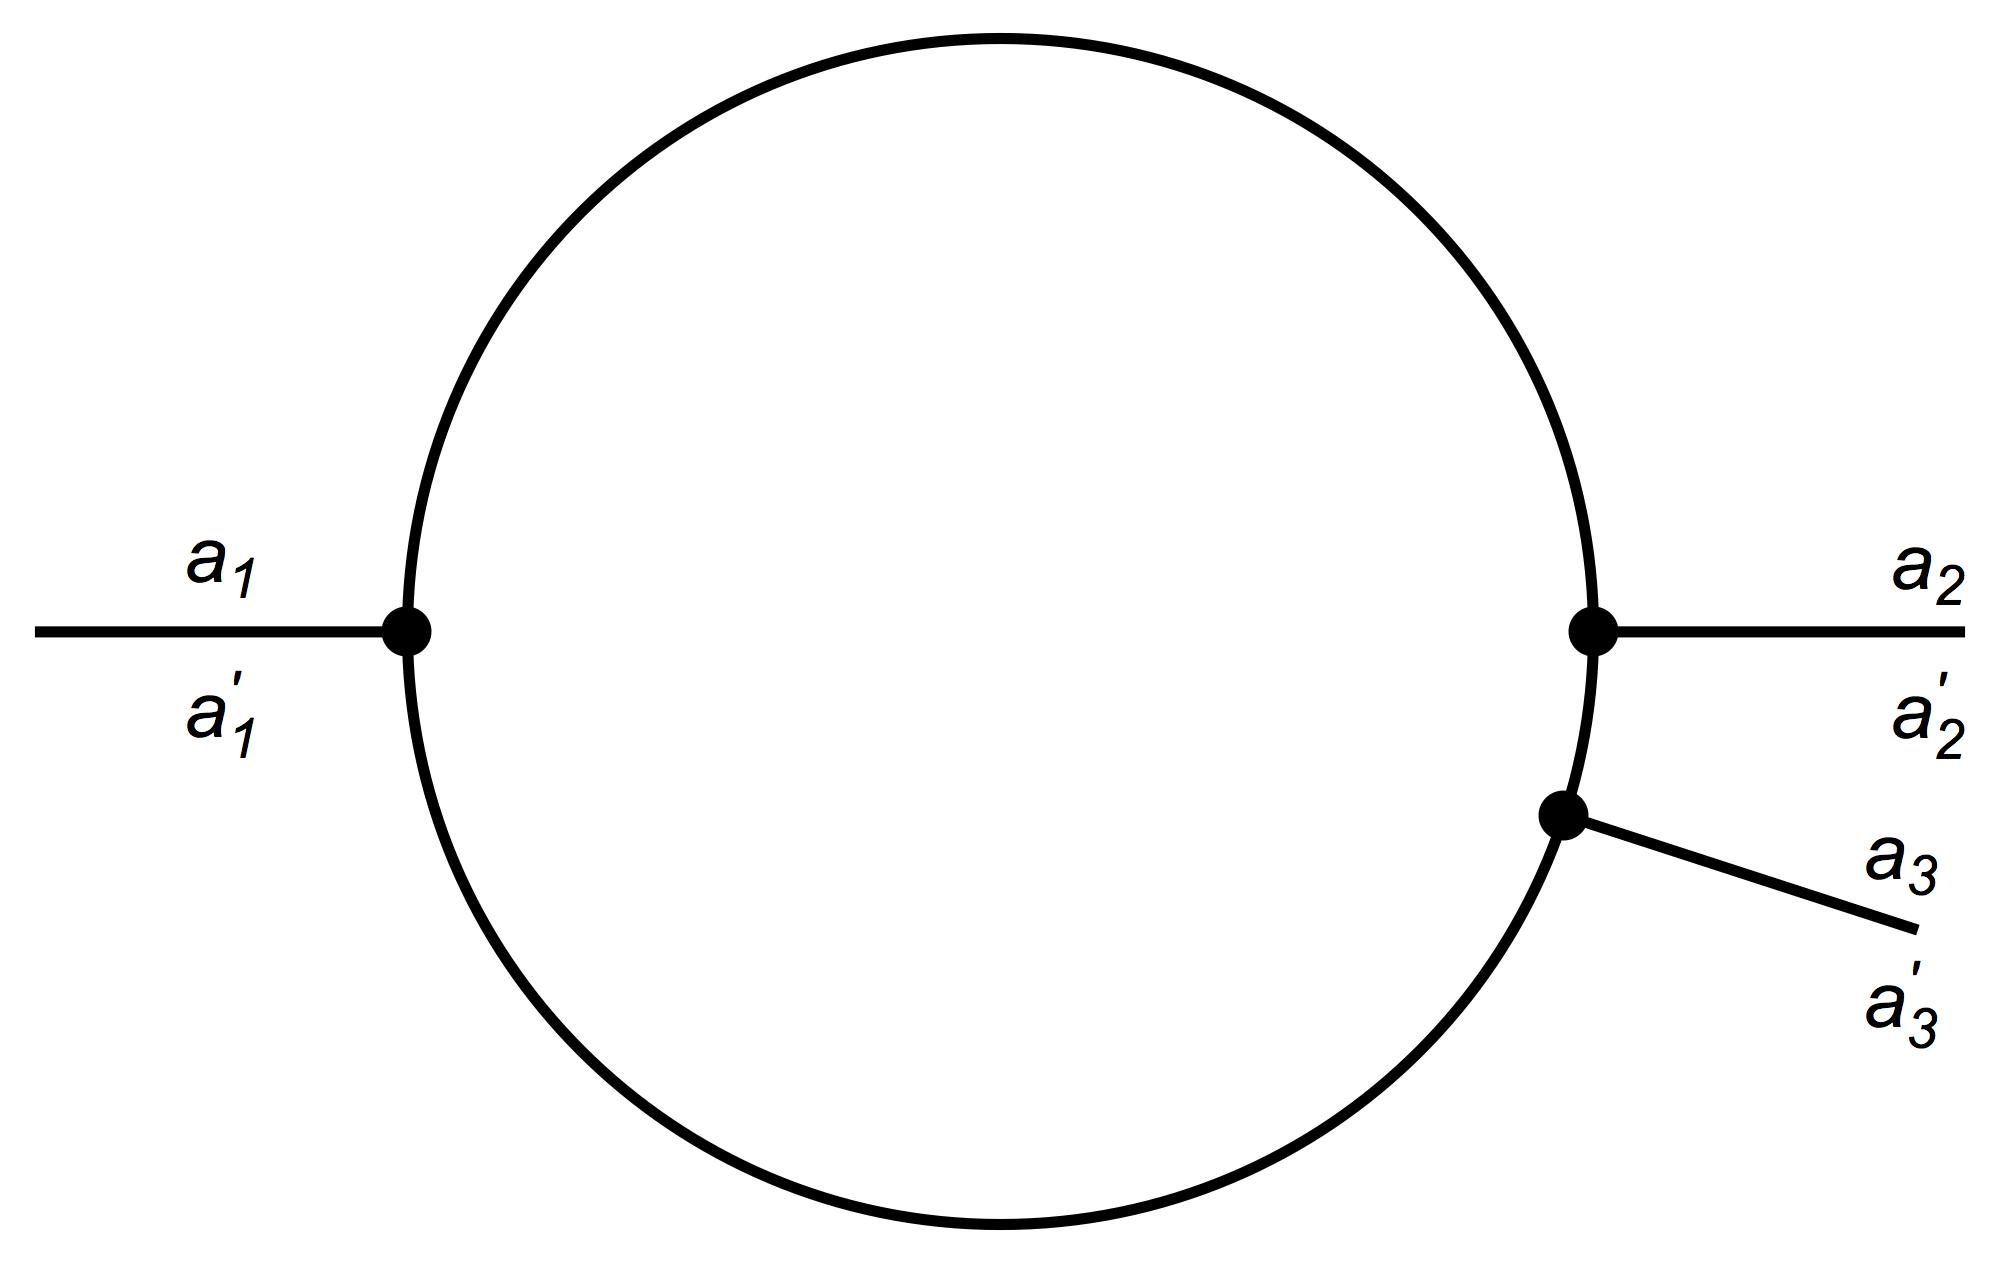
\includegraphics[width=20.0pc]{fig3.jpg}
\caption{
\small{
Scattering problem. We regard the imaging in an absolute optical instrument such as Maxwell's fish eye as a scattering problem. Radiation is fed in and out with amplitudes $a_m$ and $a_m'$ through the ports of cables that represent channels (Fig.~\ref{title}). Some of the ports act as sources, the other as detectors. For a detector port we require that $a_m=0$ while $|a_m'|^2$ gives the detected signal. We use the stereographic projection (Fig.~\ref{figstereo}) to represent the device (Fig.~\ref{title}).
}
\label{figscattering}}
\end{center}
\end{figure}
%%%

\subsection{One-dimensional model}

Let us briefly compare our Lagrangian theory with the one--dimensional model of sources and drains (and a device with $n=1$) developed earlier \cite{1D}. Consider one port at position $z=0$, and there the wave amplitudes $a=a_m$ and $a'=a_m'$ in the cable. In one dimension and for $n=1$, we can write the solution of the wave equation (\ref{w1}) as 
%%%%%%
\begin{equation}
\Psi= \begin{cases} a_+' e^{ikz} + a_- e^{-ikz} &:\quad z>0 \\ a_+ e^{ikz} + a_-' e^{-ikz} &:\quad z<0\,. 
\label{1Dfield}
\end{cases}
\end{equation}
%%%%%%
The $a_\pm$ describe the waves incoming at the port from within the device, the $a_\pm'$ the corresponding outgoing waves. We obtain from Eq.~(\ref{w1}) that $\Psi$ is continuous at $z_m$, but $\partial_z\Psi$ must jump by $g\,\partial_m \chi_m$ at $s_m=0$. We obtain from Eqs.~(\ref{fields})-(\ref{1Dfield}):
%%%%%%
\begin{gather}
a_+' + a_- = a_+ + a_-' \,, \nonumber\\
a_+' - a_- -a_+ + a_-' = g(a-a') \,,\nonumber\\
a+a' = g (a_+' + a_-) \,.
\end{gather}
%%%%%%
These relations constitute a system of three linear equations for the outgoing amplitudes in terms of the ingoing ones. One verifies that its solution agrees with Eq.~(7) of Ref.~\cite{1D}, which proves that our Lagrangian theory reproduces the one--dimensional model that has explained the experimental data \cite{Minano}. 

\subsection{Green function}

Having confirmed the validity of our Lagrangian in the case of one--dimensional propagation, we return to the case of two--dimensional imaging. We obtain from  Eqs.~(\ref{fields}) and (\ref{chi}):
%%%%%%
\begin{equation}
a_m + a_m' = g\Psi(z_m) \,.
\label{amp}
\end{equation}
%%%%%%
We assume that the field in the device is only generated through the cables; there is no initial field remaining inside. Then we can write the solution of Eq.~(\ref{w1}) in terms of the Green function $G(z_,z_0)$ as
%%%%%%
\begin{equation}
\Psi = ikg\sum_m G(z,z_m) \,(a_m-a_m') \,.
\label{field}
\end{equation}
%%%%%%
For Maxwell's fish eye and, equivalently, the surface of the sphere, the Green function is given by the expression \cite{Leo2}
%%%%%%
\begin{equation}
G = \frac{P_\nu(\zeta_m)}{4\sin\nu\pi} 
\label{green}
\end{equation}
%%%%%%
in terms of the Legendre function $P_\nu$ \cite{Erdelyi} with index
%%%%%%
\begin{equation}
\nu = \frac{1}{2} \left(\sqrt{4k^2+1} - 1\right) \,.
\end{equation}
%%%%%%
At resonances the $\nu$ are integer; the resonances correspond to the standing waves on the surface of the sphere. The $\zeta_m$ depend on the coordinate $z$ and the position $z_m$ of the $m$-th port \cite{Leo2}:
%%%%%%
\begin{equation}
\zeta_m = \frac{|z'|^2-1}{|z'|^2+1} \,,\quad z' = \frac{z-z_m}{z_m^*z+1} \,.
\label{zeta}
\end{equation}
%%%%%%
If the fish eye is surrounded by a mirror (Fig.~\ref{title}) at $|z|=1$, the stereographic projection of the Equator of the sphere, we need to use the Green function \cite{Fish,Leo2}
%%%%%%
\begin{equation}
G' = G(z,z_0) - G(1/z^*,z_0) \,.
\end{equation}
%%%%%%
The mirror serves the purpose of making Maxwell's fish eye practically applicable, as it confines the refractive--index profile of Eq.~(\ref{maxwell}) within $|z|\le1$ where the refractive index varies maximally by a factor of two. Here we are primarily interested in the fundamental capabilities and limitations of perfect imaging with interacting sources and drains, and so we only consider Maxwell's original fish eye with Green function of Eq.~(\ref{green}), but our results are easily generalizable. 

Note that near a port the Green function must diverge logarithmically \cite{Fish}, because the port acts as a delta--function source for a two--dimensional wave. For Maxwell's fish eye we obtain for $z\sim z_m$ where $\zeta_m\sim-1$ the asymptotics
%%%%%%
\begin{equation}
G \sim \frac{1}{4\pi} \bigg[ \ln \left(\frac{\zeta_m+1}{2}\right) + 2\gamma + 2\psi(\nu+1) +\pi \cot \nu\pi\bigg]
\label{asymp}
\end{equation}
%%%%%%
where $\gamma$ denotes Euler's constant and $\psi$ the digamma function \cite{Erdelyi}. The logarithmic divergence is a consequence of the dimensionality mismatch between the device and the cables leading radiation to and from --- two--dimensional radiation originates or disappears at the ports of entry of one--dimensional cables. In practice, we would regularize the divergence, requiring, for example, that the cables have a small but finite diameter. However, in this paper we are mostly concerned with the behavior of the system near a resonance where $\nu$ tends to an integer. Here the $\cot\nu\pi$ term in Eq.~(\ref{asymp}) dominates over the logarithmic term if the latter is regularized. We regard the logarithm as a good approximation for a constant, and use simply
%%%%%%
\begin{equation}
G \sim \frac{\cot \nu\pi}{4} \quad\mbox{for}\quad z\sim z_m\,.
\label{asymptoto}
\end{equation}
%%%%%%
Now we are perfectly prepared to tackle the problem of perfect imaging in Maxwell's fish eye with mutually interacting sources and drains.

\section{Analysis}

\subsection{Scattering matrix}

The amplitudes $a_m$ describe the incoming waves at the ports, the $a_m'$ the outgoing waves (Fig.~\ref{figscattering}). We wish to relate the vectors $\bm{a}$ and $\bm{a}'$ of the $a_m$ and $a_m'$ as
%%%%%%
\begin{equation}
\bm{a}' = S \bm{a}
\label{scattering}
\end{equation}
%%%%%%
where $S$ denotes the scattering matrix. We notice that Eqs.~(\ref{amp}) and (\ref{field}) evaluated at $z=z_l$ establish a closed system of linear equations for $a_m'$. The solution is going to be of the form of Eq.~(\ref{scattering}) and, therefore, will give the scattering matrix. Equation (\ref{field}) at $z=z_l$ depends on the Green function, Eq.~(\ref{green}), at $\zeta_{ml}=\zeta_m(z_l) =\zeta_{lm}$. Note that  $\zeta_{ml}=-1$ for $l=m$ (the port interacting with itself) where the Green function diverges, unless it is regularized. In this case we use the asymptotics of Eq.~(\ref{asymptoto}) for the Green function.

It is convenient to express the linear system of Eqs.~(\ref{amp}) and (\ref{field}) at $z=z_l$ in terms of the matrix
%%%%%%
\begin{equation}
W_{ml} = \begin{cases} \cos\nu\pi - i\sigma\sin\nu\pi &: \quad l=m \\ P_\nu(\zeta_{ml}) &:\quad l \neq m \end{cases}
\label{W}
\end{equation}
%%%%%%
with the parameter
%%%%%%
\begin{equation}
\sigma = \frac{4}{g^2k} \,.
\label{sigma}
\end{equation}
%%%%%%
We see that the linear system appears as
%%%%%%
\begin{equation}
W\bm{a}' = W^*\bm{a} \,,
\label{linear}
\end{equation}
%%%%%%
and hence 
%%%%%%
\begin{equation}
S = W^{-1} W^* \,.
\label{S}
\end{equation}
%%%%%%
As the scattering matrix is given by the ratio between $W^*$ and $W$, it crucially depends on the imaginary part of $W$. We see from Eq.~(\ref{W}) that
%%%%%%
\begin{equation}
W = V - i\sigma \sin\nu\pi \, \mathbb{1} \,,\quad V=\left.W\right|_{\sigma=0} 
\label{WV}
\end{equation}
%%%%%%
where $V$ is a real matrix. At a resonance where $\nu\in\mathbb{N}$ the imaginary part vanishes; $S=\mathbb{1}$ if $\det V \neq 0$, which means the outgoing radiation is equal to the incoming radiation --- the device rejects all incident waves and reflects them. However, in the case of imaging, $\det V$ turns out to vanish, and so the limit $\nu\rightarrow\mbox{integer}$ is subtle.

Near a resonance, the calculation of the scattering matrix becomes numerically delicate. It is advisable to compute $S$ with the help of the eigenvalues and eigenvectors of $V$. We see from Eqs.~(\ref{zeta}), (\ref{W}) and (\ref{WV}) that $V$ is a symmetric real matrix. Hence $V$ has real eigenvalues $V_m$ and an orthogonal system of eigenvectors. We express $V$ as 
%%%%%%
\begin{equation}
V=R^T{\rm diag} (V_m) R 
\end{equation}
%%%%%%
in terms of the rotation matrix $R$ of the normalized eigenvectors. From Eq.~(\ref{WV}) follows that
%%%%%%
\begin{equation}
W=R^T{\rm diag} (W_m) R 
\end{equation}
%%%%%%
with the eigenvalues
%%%%%%
\begin{equation}
W_m = V_m - i\sigma \sin\nu\pi \,.
\end{equation}
%%%%%%
Since $R$ is real, we obtain from Eq.~(\ref{S}) for the scattering matrix
%%%%%%
\begin{equation}
S=R^T{\rm diag} (W_m^*/W_m) R \,,
\label{Sresult}
\end{equation}
%%%%%%
which is a numerically more stable expression than Eq.~(\ref{S}), although it may still require high-precision arithmetics near a resonance. We also see from Eq.~(\ref{Sresult}) that $S$ is unitary, as one does expect: we are dealing with a passive device where the total intensity is conserved, $\bm{a}'^*\cdot \bm{a}'=\bm{a}^*\cdot \bm{a}$, which implies that $S$ is unitary, $S^{-1}=S^\dagger$. Furthermore, we see from Eq.~(\ref{Sresult}) that $S^{-1}=S^*$ and so obtain from unitarity $S=S^T$: the scattering matrix is symmetric.

\subsection{Single source, single drain}

Consider the case \cite{MinanoSim,Minano} when a single source is facing a moveable single detector (Fig.~\ref{1o1}). Without loss of generality, we put the source at the South Pole of the sphere ($\theta_1=\pi$) and the drain an angle $\delta$ away from the North Pole ($\theta_2=\delta$, $\phi_2=0$). For simplicity, we only consider the wave propagation along the circle $\phi=0$ where, according to Eqs.~(\ref{stereo}) and (\ref{zeta}),
%%%%%%
\begin{equation}
\zeta_m=-\cos(\theta-\theta_m) \,.
\label{zetam}
\end{equation}
%%%%%%
%%%
\begin{figure}[h]
\begin{center}
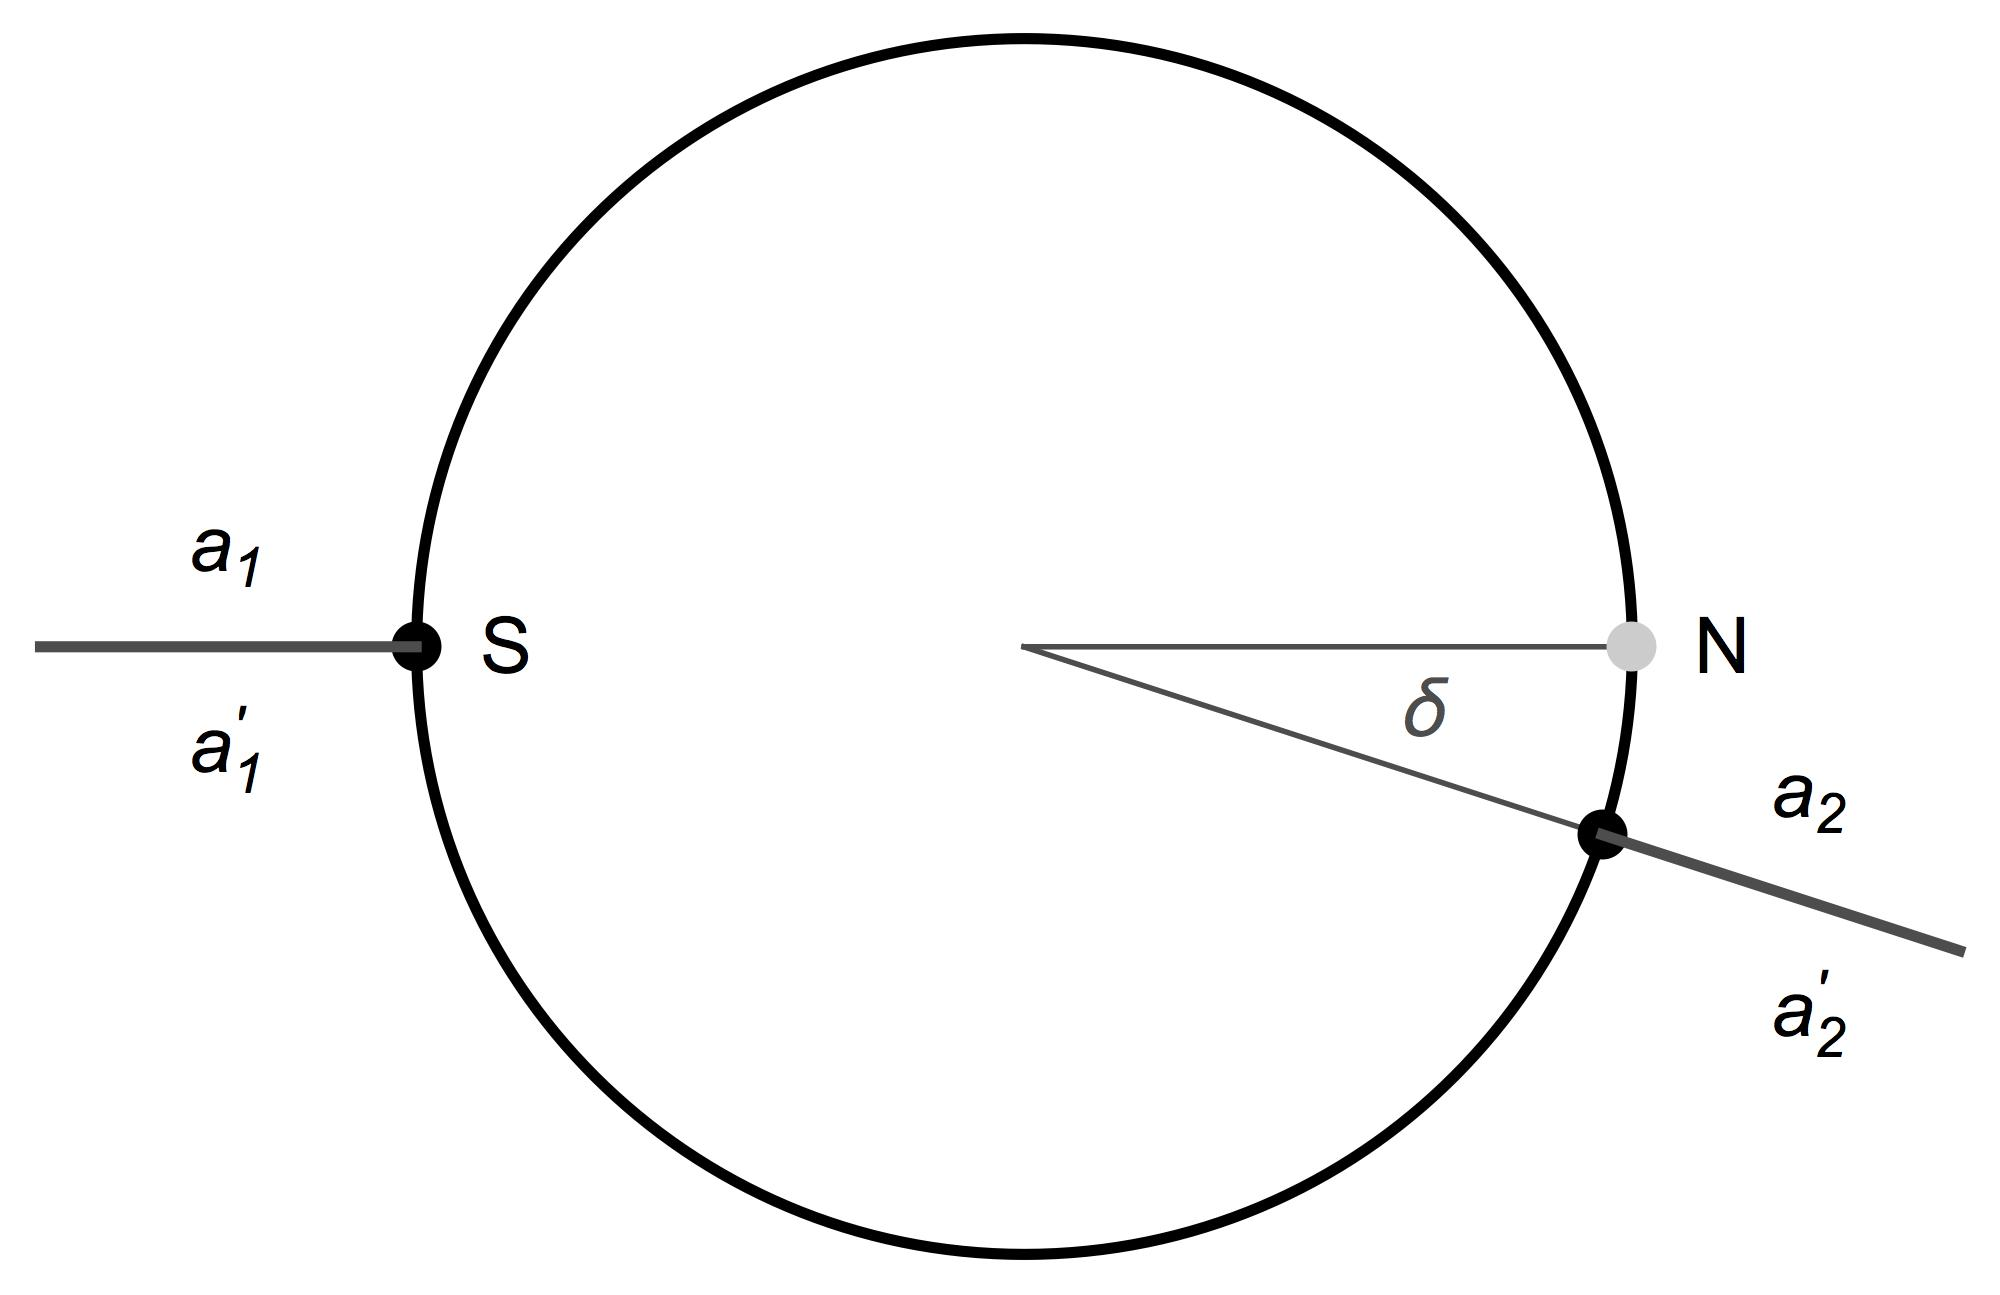
\includegraphics[width=20.0pc]{fig4.jpg}
\caption{
\small{
Single source, single drain --- the setup of experiment \cite{Minano}. Radiation incident at the source S is scanned with a mobile drain the angle $\delta$ away from N. (We turned the sphere of Fig.~\ref{figstereo}). 
}
\label{1o1}}
\end{center}
\end{figure}
%%%

Requiring $a_1=1$ (unit source) and $a_2=0$ (drain) we obtain from the solution of the linear system of Eq.~(\ref{linear}) with matrix $W$ defined in Eq.~(\ref{W}):
%%%%%%
\begin{eqnarray}
a_1' &=& \frac{P_\nu(\cos\delta)^2 - \cos^2\nu\pi - \sigma^2\sin^2\nu\pi}{P_\nu(\cos\delta)^2 - (\cos\nu\pi - i\sigma\sin\nu\pi)^2} \,,
\nonumber\\
a_2' &=& \frac{2i\sigma\sin\nu\pi\,P_\nu(\cos\delta)}{P_\nu(\cos\delta)^2 - (\cos\nu\pi - i\sigma\sin\nu\pi)^2} \,.
\label{as}
\end{eqnarray}
%%%%%%
The intensity $|a_2'|^2$ describes the transmission of the device through the detector port. We see that $a_2'$ vanishes at a resonance where $\nu\in\mathbb{N}$, unless $\delta=0$. The transmission shows the Mi\~{n}ano dips \cite{MinanoSim,Minano} characteristic of absolute optical instruments \cite{1D}: when the radiation is resonant, a displacement of the detector, however small, will extinguish the transmission; the incident radiation is completely reflected. For $\delta=0$, on the other hand, $a_2'$ tends to $(-1)^\nu$ at resonance: for perfect alignment of source and drain all incident radiation is transmitted. This on-off behaviour may be useful in scanning a single source with arbitrary precision from some distance away.

Figure \ref{minanodips} shows the transmission versus wave index $\nu$. The figure agrees well with the transmission curve of the simple one--dimensional model \cite{1D} and with the experiment \cite{Minano}, apart from a tiny shift of the resonance frequencies that is probably due to the finite sizes of the source and drain. The Mi\~{n}ano dips are narrow features in the transmission curve; we characterize their width by 
%%%%%%
\begin{equation}
\left.
\frac{1}{2}\, \frac{\partial^2|a_2'|^2}{\partial\nu^2}\right|_{\nu\in\mathbb{N}} = \left(\frac{2\pi \sigma P_\nu(\cos\delta)}{P_\nu(\cos\delta)^2 -1}\right)^2
\end{equation}
%%%%%%
that scales like $\delta^{-4}$ for small $\delta$. Minute deviations of the drain are thus detectable near resonance.

%%%
\begin{figure}[h]
\begin{center}
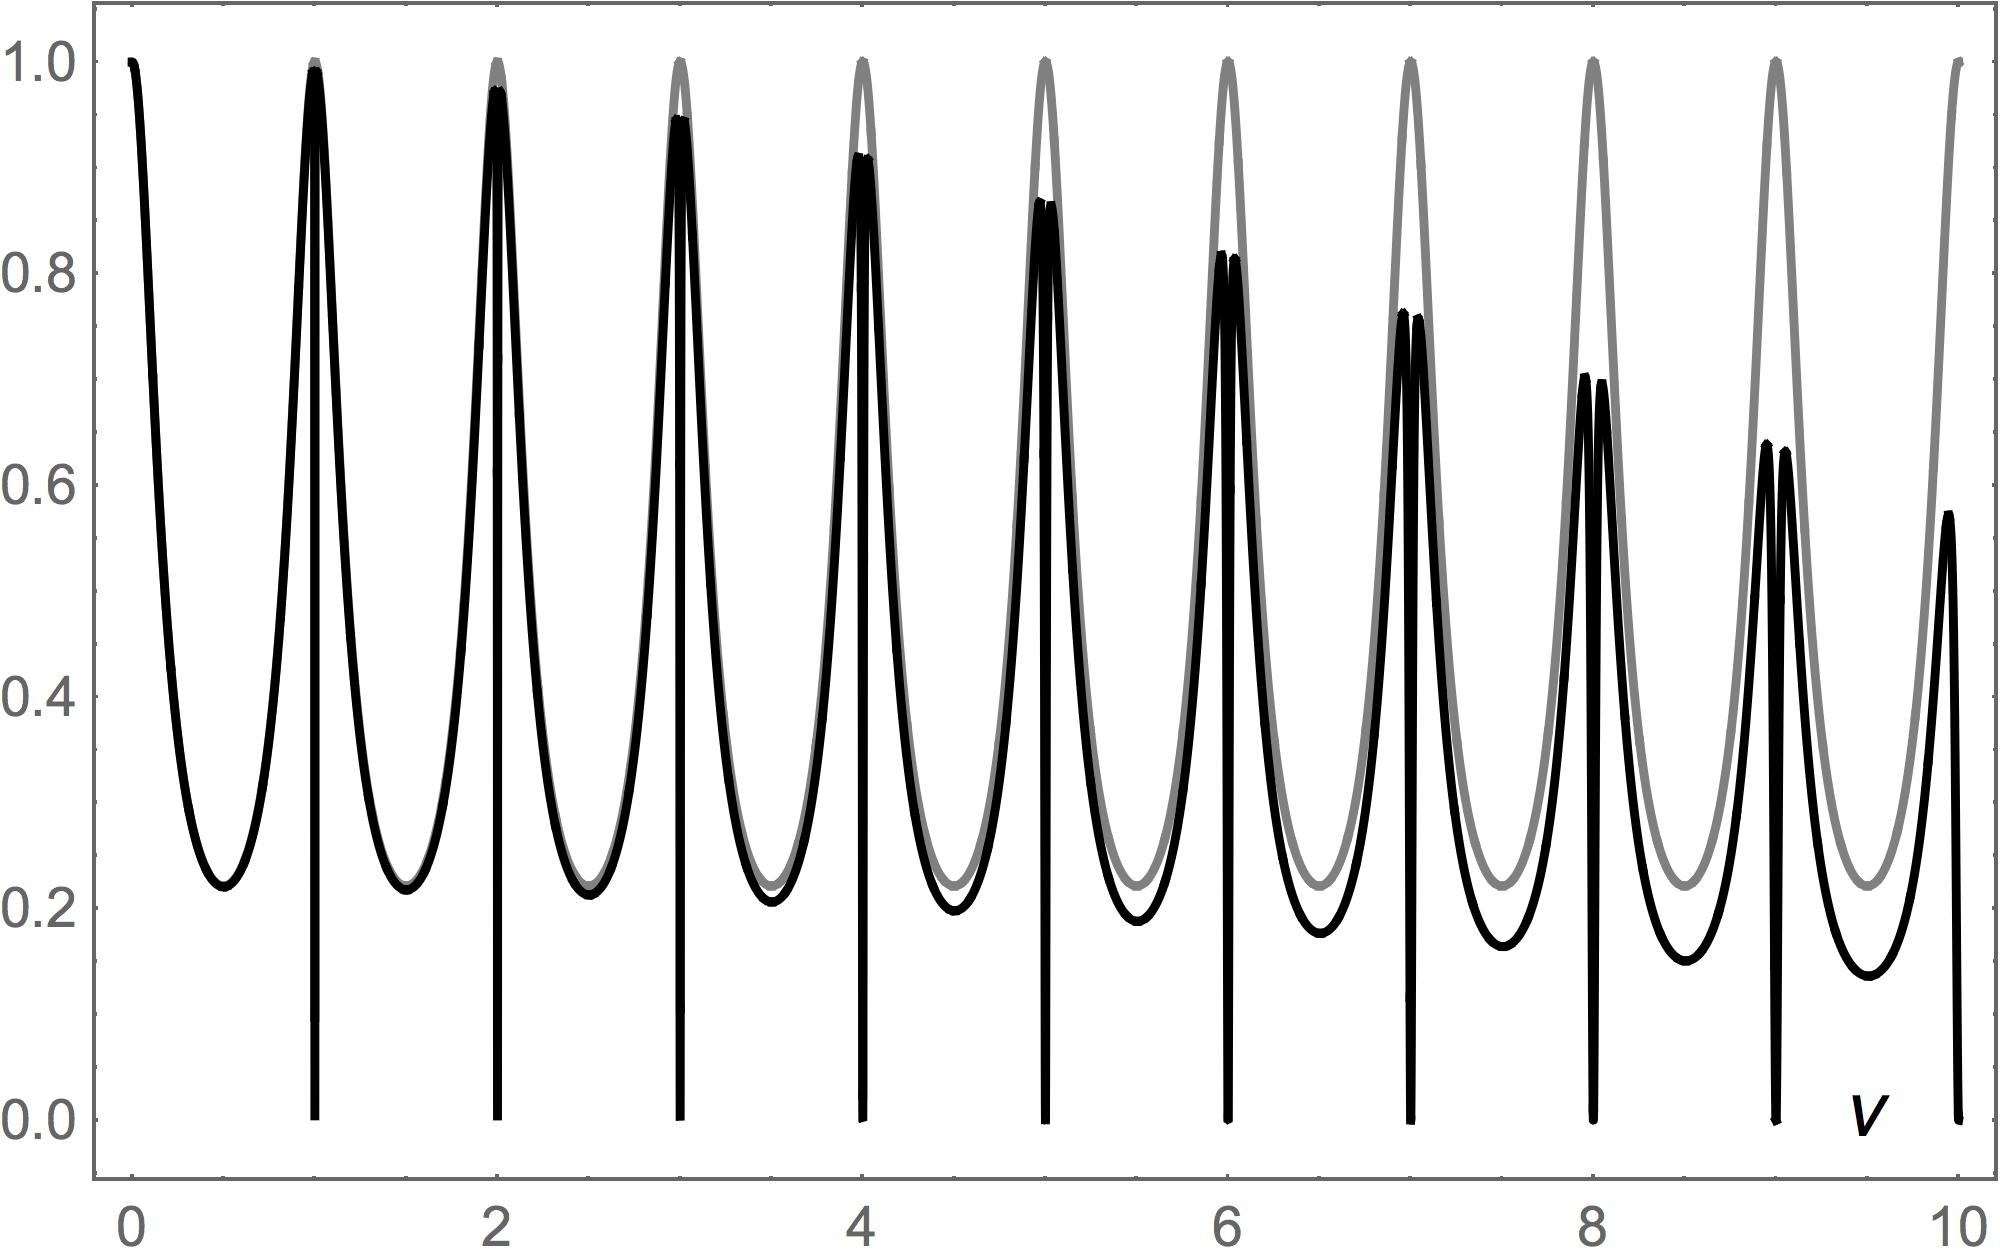
\includegraphics[width=20.0pc]{fig5.jpg}
\caption{
\small{
Mi\~{n}ano dips with the setup of Fig.~\ref{1o1}. Transmission of a single source through Maxwell's fish eye to a single drain, {\it i.e.} $|a_2'|^2$ of Eq.~(\ref{as}) plotted as a function of $\nu$. Black curve: the drain is misaligned by the angle $\delta=0.1$. Gray curve: $\delta=0$, the drain is at the correct imaging position. In both cases we take $\sigma=4.0$. The figure shows the typical Fabry-Perot resonances of the device, but also, for the misaligned drain, sharp drops at the resonances ($\nu\in\mathbb{N}$), the Mi\~{n}ano dips.
}
\label{minanodips}}
\end{center}
\end{figure}
%%%
 
Consider the case of perfect alignment of source and drain, $\delta=0$, for variable $\nu$. We obtain from Eq.~(\ref{as})
%%%%%%
\begin{equation}
|a_2'|^2 = \frac{1}{\cos^2\nu\pi + T^{-2}\sin^2\nu\pi} \,,\quad
T= \frac{2}{\sigma + \sigma^{-1}} \,.
\end{equation}
%%%%%%
The device behaves like a typical Fabry--Perot resonator with average transmission 
%%%%%%
\begin{equation}
\int_m^{m+1} |a_2'|^2 d\nu = T \,.
\end{equation}
%%%%%%
At resonance, it transmits perfectly. Out of resonance, the transmission is reduced due to coupling losses, unless $\sigma=1$ that we regard as the case of perfect coupling.

Finally, we calculate the field $\Psi$ for the case of perfect alignment. We obtain from Eqs.~(\ref{field}), (\ref{green}), (\ref{sigma}) and (\ref{as}) for $\delta=0$ the field
%%%%%%
\begin{equation}
\Psi = \frac{i\sqrt{k}}{\pi}\,\tau\eta\, e^{i\nu\pi} \left[Q_\nu(\zeta) + \rho\, e^{i\nu\pi} Q_\nu(-\zeta)\right]
\label{psi}
\end{equation}
%%%%%%
in terms of the Legendre functions $Q_\nu$ (defined on the branch cut \cite{Erdelyi}),
%%%%%%
\begin{equation}
Q_\nu(\zeta) = \frac{\pi}{2}\,\frac{e^{-i\nu\pi}P_\nu(\zeta) - P_\nu(-\zeta)}{\sin\nu\pi} \,,
\end{equation}
%%%%%%
and the coefficients
%%%%%%
\begin{eqnarray}
\tau &=& \frac{2\sqrt{\sigma}}{\sigma+1} \,,
\nonumber\\
\rho &=& \frac{\sigma - 1}{\sigma +1} \,,
\nonumber\\
\eta &=& \frac{1}{1-e^{2i\nu\pi}\rho^2} \,.
\end{eqnarray}
%%%%%%
Note that $e^{i\nu\pi}Q_\nu(\zeta)$ describes a running wave from the source to the drain \cite{Fish}, the outgoing wave; $Q_\nu(-\zeta)$ corresponds to a wave running back from the drain to the source, the ingoing wave. Note also that $Q_\nu$ is well--behaved for $\nu\rightarrow\mbox{integer}$. We interpret $\tau$ and $\rho$ as the transmission and reflection coefficients of the ports, with $\tau^2+\sigma^2=1$. The factor $\eta$ sums up the geometric series 
%%%%%%
\begin{equation}
\eta = \sum_{m=0}^\infty e^{2im\nu\pi}\rho^{2m}
\end{equation}
%%%%%%
of all the reflections and phase factors during the roundtrips in the device. The field of Eq.~(\ref{psi}) thus describes the characteristic behavior of a wave injected with transmittance $\tau$ that accumulates a phase shift of $\nu\pi$ from source to drain, is reflected with reflectance $\rho$, gains the phase factor $\nu\pi$ from drain to source where it is reflected again {\it etc.}, until it is recorded at the drain. In the case of perfect coupling we obtain the sole running wave $e^{i\nu\pi}Q_\nu(\zeta)$ characteristic of perfect imaging in the two--dimensional Maxwell fish eye \cite{Fish}.

\subsection{Single source, multiple drains}

In Sec.~III B we investigated in detail a single source observed with a single, movable detector in Maxwell's fish eye. Imagine now the source faces an array of $M$ detectors. The source we put at port 1, the drains at the remaining ports. Consider the field $\Psi$ given by Eq.~(\ref{field}) with the Green function of Eq.~(\ref{green}) close to a resonance ($\nu\in\mathbb{N}$) where we might expect perfect imaging. The field must remain finite at resonance, but Eq.~(\ref{field}) diverges when $\nu\rightarrow\mbox{integer}$, unless 
%%%%%%
\begin{equation}
\sum_{m=1}^{M+1} P_\nu (\zeta_m)\,(a_m-a_m') = 0 \,.
\label{null}
\end{equation}
%%%%%%
Suppose that all the drains are misaligned and also that all the $P_\nu (\zeta_m)$ are linearly independent functions. It follows that 
%%%%%%
\begin{equation}
a_1'=a_1\,,\quad a_m'=a_m=0 \,.
\end{equation}
%%%%%%
The device rejects the radiation fed in at the source; none of the detectors fires. 

Suppose now one drain is aligned with the source, say port number 2. In this case $\zeta_2=-\zeta_1$ and $P_\nu(-\zeta)=(-1)^\nu P_\nu(\zeta)$ for $\nu\in\mathbb{N}$. We thus have
%%%%%%
\begin{equation}
P_\nu(\zeta_1)\left[a_1-a_1'-(-1)^\nu a_2'\right]-\sum_{m=3}^{M+1} P_\nu (\zeta_m)\,a_m' = 0 \,.
\label{null1}
\end{equation}
%%%%%%
We get
%%%%%%
\begin{equation}
a_m'=0 \quad\mbox{for}\quad m>2 \,;
\end{equation}
%%%%%%
none of the auxiliary detectors fire. The problem reduces itself to the problem of a single drain aligned to a single source, our previous case of Sec.~III B. There we have seen that 
%%%%%%
\begin{equation}
a_1'=0\,,\quad a_2'= (-1)^\nu a_1
\end{equation}
%%%%%%
at resonance when $\nu\in\mathbb{N}$. The detector array thus perfectly discriminates between the correct image position and the incorrect ones, irrespective of the distance between the detectors, {\it i.e.} not affected by the diffraction limit \cite{Abbe,BornWolf}.

Figure \ref{minano2} shows the simplest case: one source facing one aligned and also one misaligned drain (similar to Fig.~\ref{title}). We see that the transmission of the misaligned drain exhibits the characteristic Mi\~{n}ano dips \cite{1D}, while the transmittance of the aligned drain becomes perfect at the resonances.

%%%
\begin{figure}[h]
\begin{center}
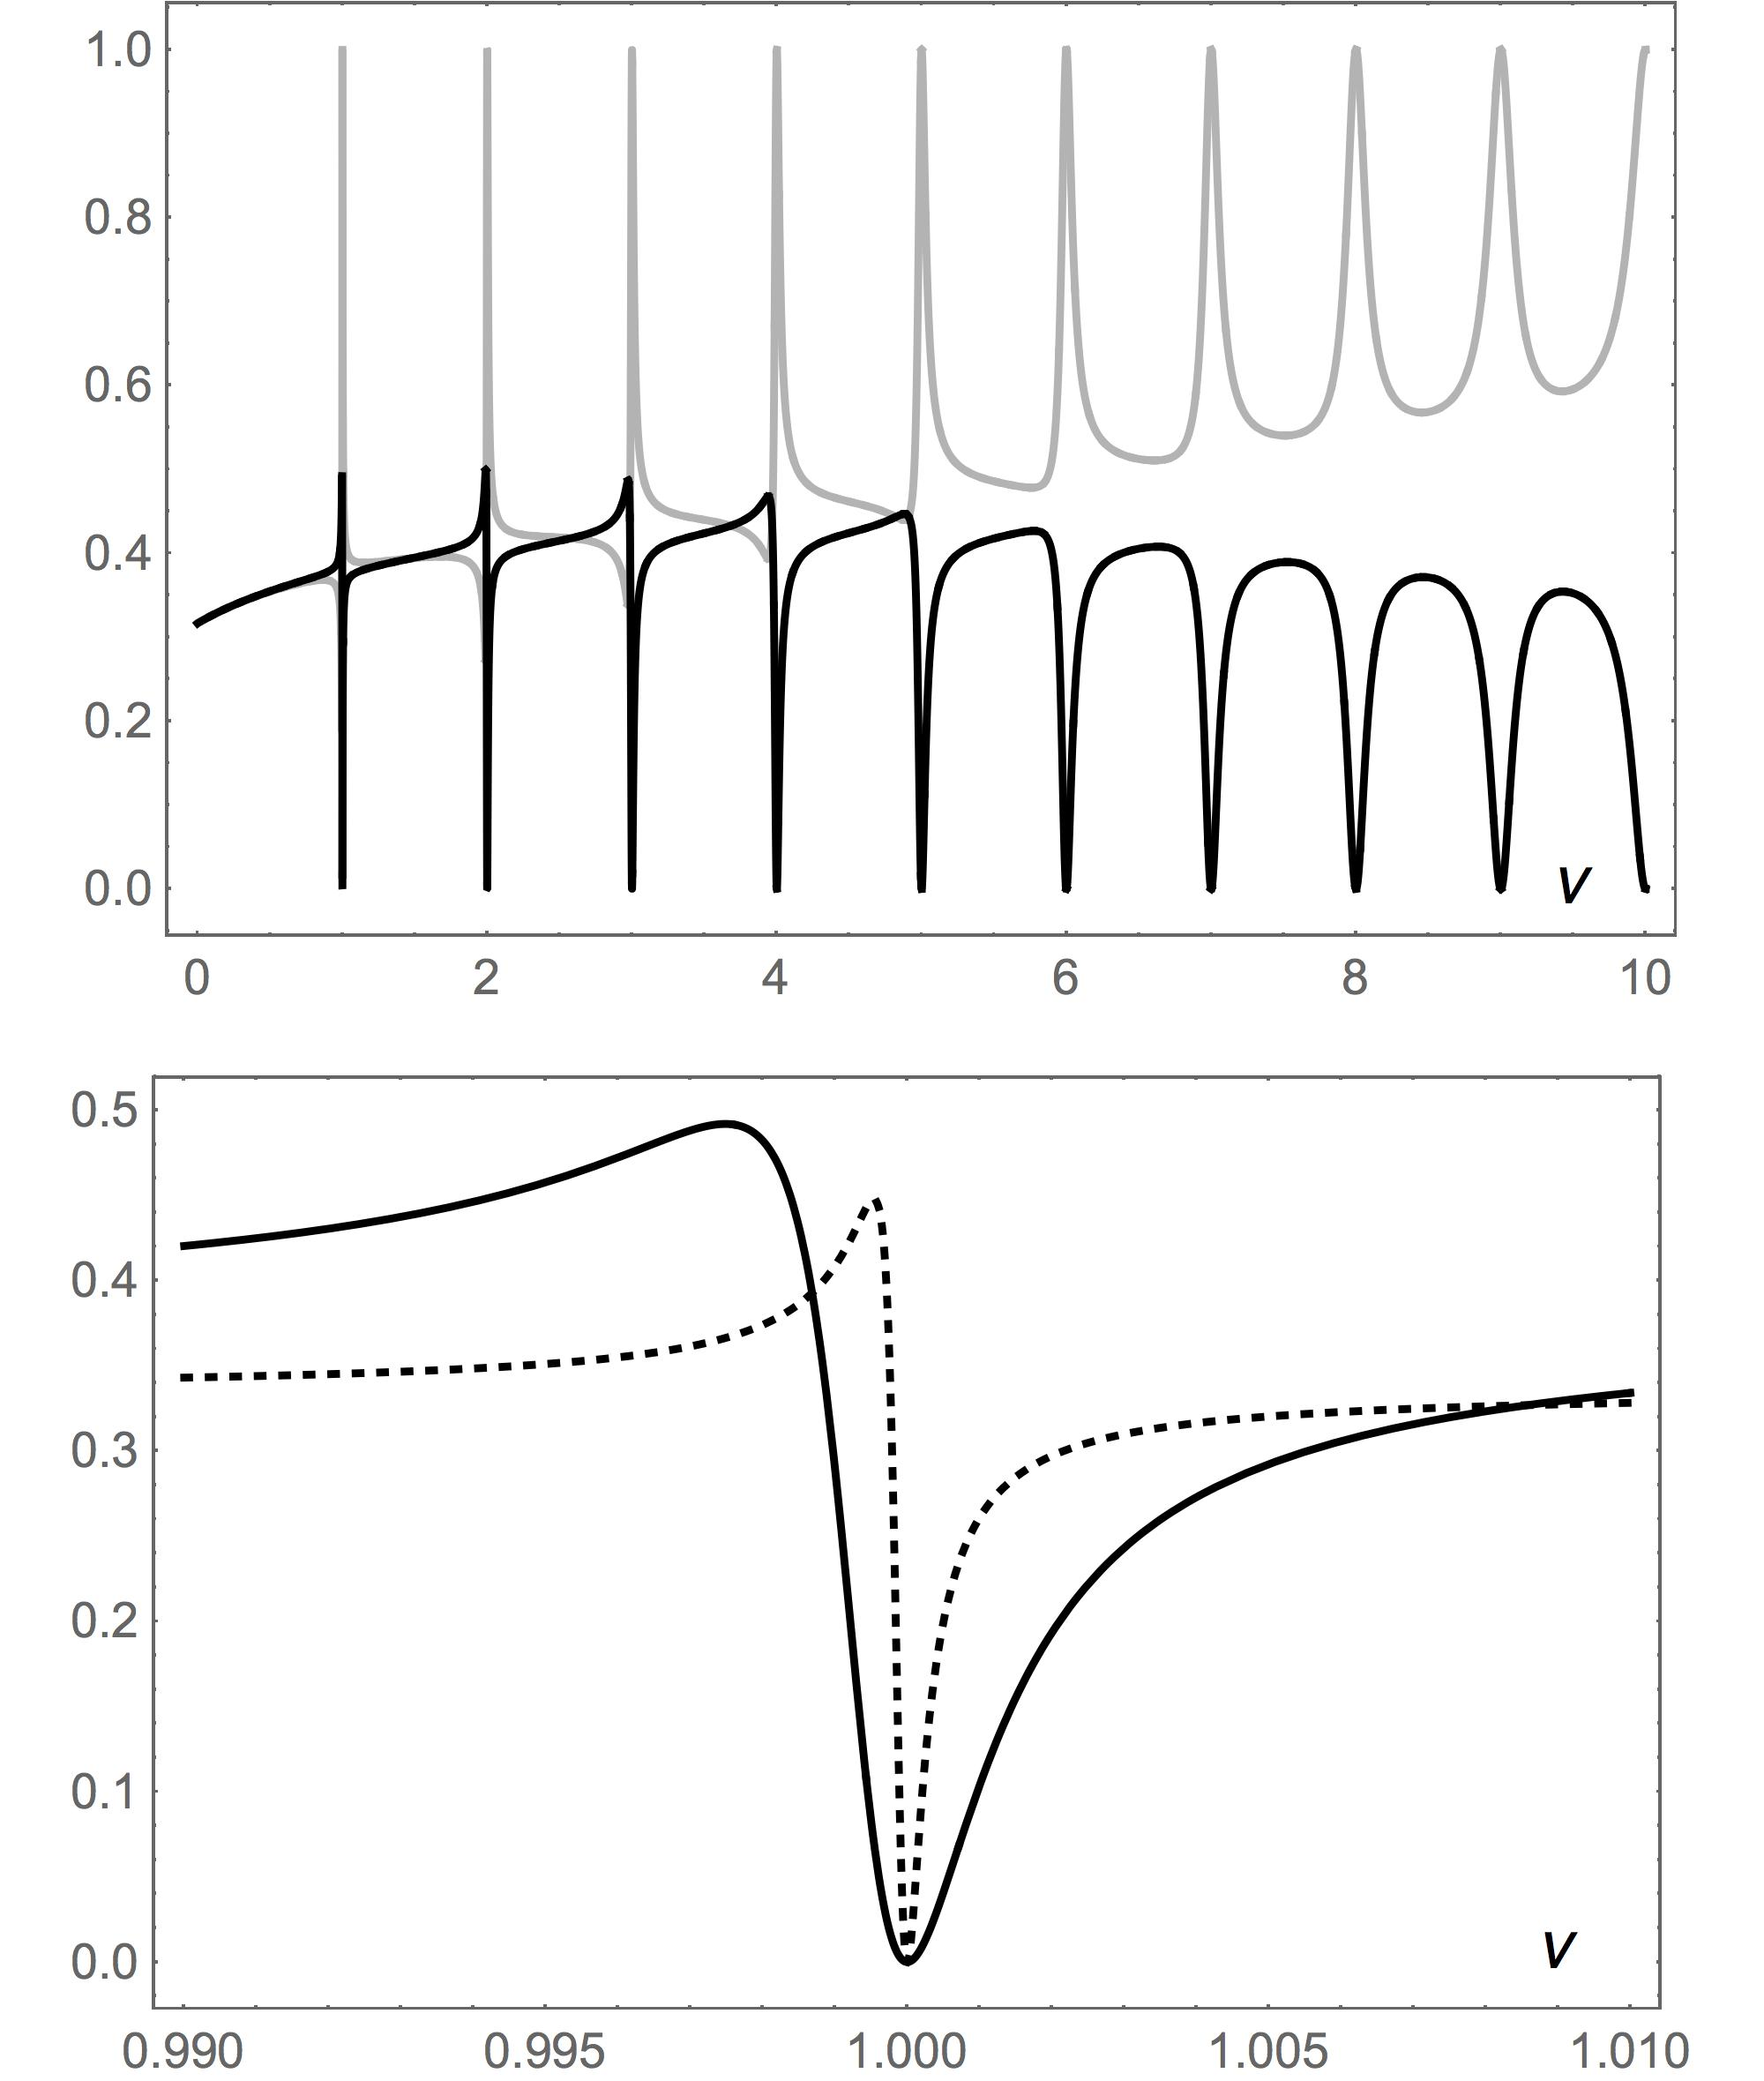
\includegraphics[width=20.0pc]{fig6.jpg}
\caption{
\small{
Mi\~{n}ano dips for multiple drains. Transmission of a single source to two drains (similar to Fig.~\ref{title}), one at the correct imaging position and the other misaligned by the angle $\delta$ on the virtual sphere. We assume the case of perfect coupling, $\sigma=1$. Top: the black curve shows the transmission through the misaligned drain ($\delta=0.1$), the light--gray curve the one through the aligned drain. The figure exhibits sharp Mi\~{n}ano dips for subwavelength separation, lesser sharp dips and a growing gap between the two transmission curves for $\nu\delta>1/2$. Bottom: transmission curve of the misaligned drain around a Mi\~{n}ano dip for $\delta=0.1$ (solid curve) and $\delta=0.05$ (dotted). One sees how the dip narrows for smaller drain separations. 
}
\label{minano2}}
\end{center}
\end{figure}
%%%

However, we must make one important qualification. We need to assume that the $P_\nu(\zeta_m)$ for all the detectors are linearly independent. However, the function space of the stationary waves on the unit sphere is $(\nu+1)$--dimensional, for the following reason: the space is as dimensional as the quantum--mechanical state space of an angular momentum with quantum number $\nu$ \cite{LL3} restricted to real wavefunctions. We thus need to require that the number of detectors does not exceed $\nu+1$, the number of linearly--independent waves at resonance.  

\subsection{Multiple sources}

Which ones of the imaging properties of the single source will remain valid for multiple sources? Consider first $M$ sources and one moveable detector, the exact opposite of the situation investigated in Sec.~III C. The sources are assumed to be coherent; incoherent sources are statistical ensembles of single sources. We assign port 1 to the detector and the other ports to the sources, and assume resonance. We obtain from Eq.~(\ref{null}) that none of the sources is able to inject radiation, $a_m'=a_m$, unless the detector is aligned to one of them. In this case, the corresponding source transmits all of its radiation to the detector. At exact resonance this effect is independent of the distances between the sources (detuned from resonance it will be): the detector is thus able to scan near--field features from a far--field distance, and without the need of switching on the sources selectively \cite{RMP}.

%%%
\begin{figure}[h]
\begin{center}
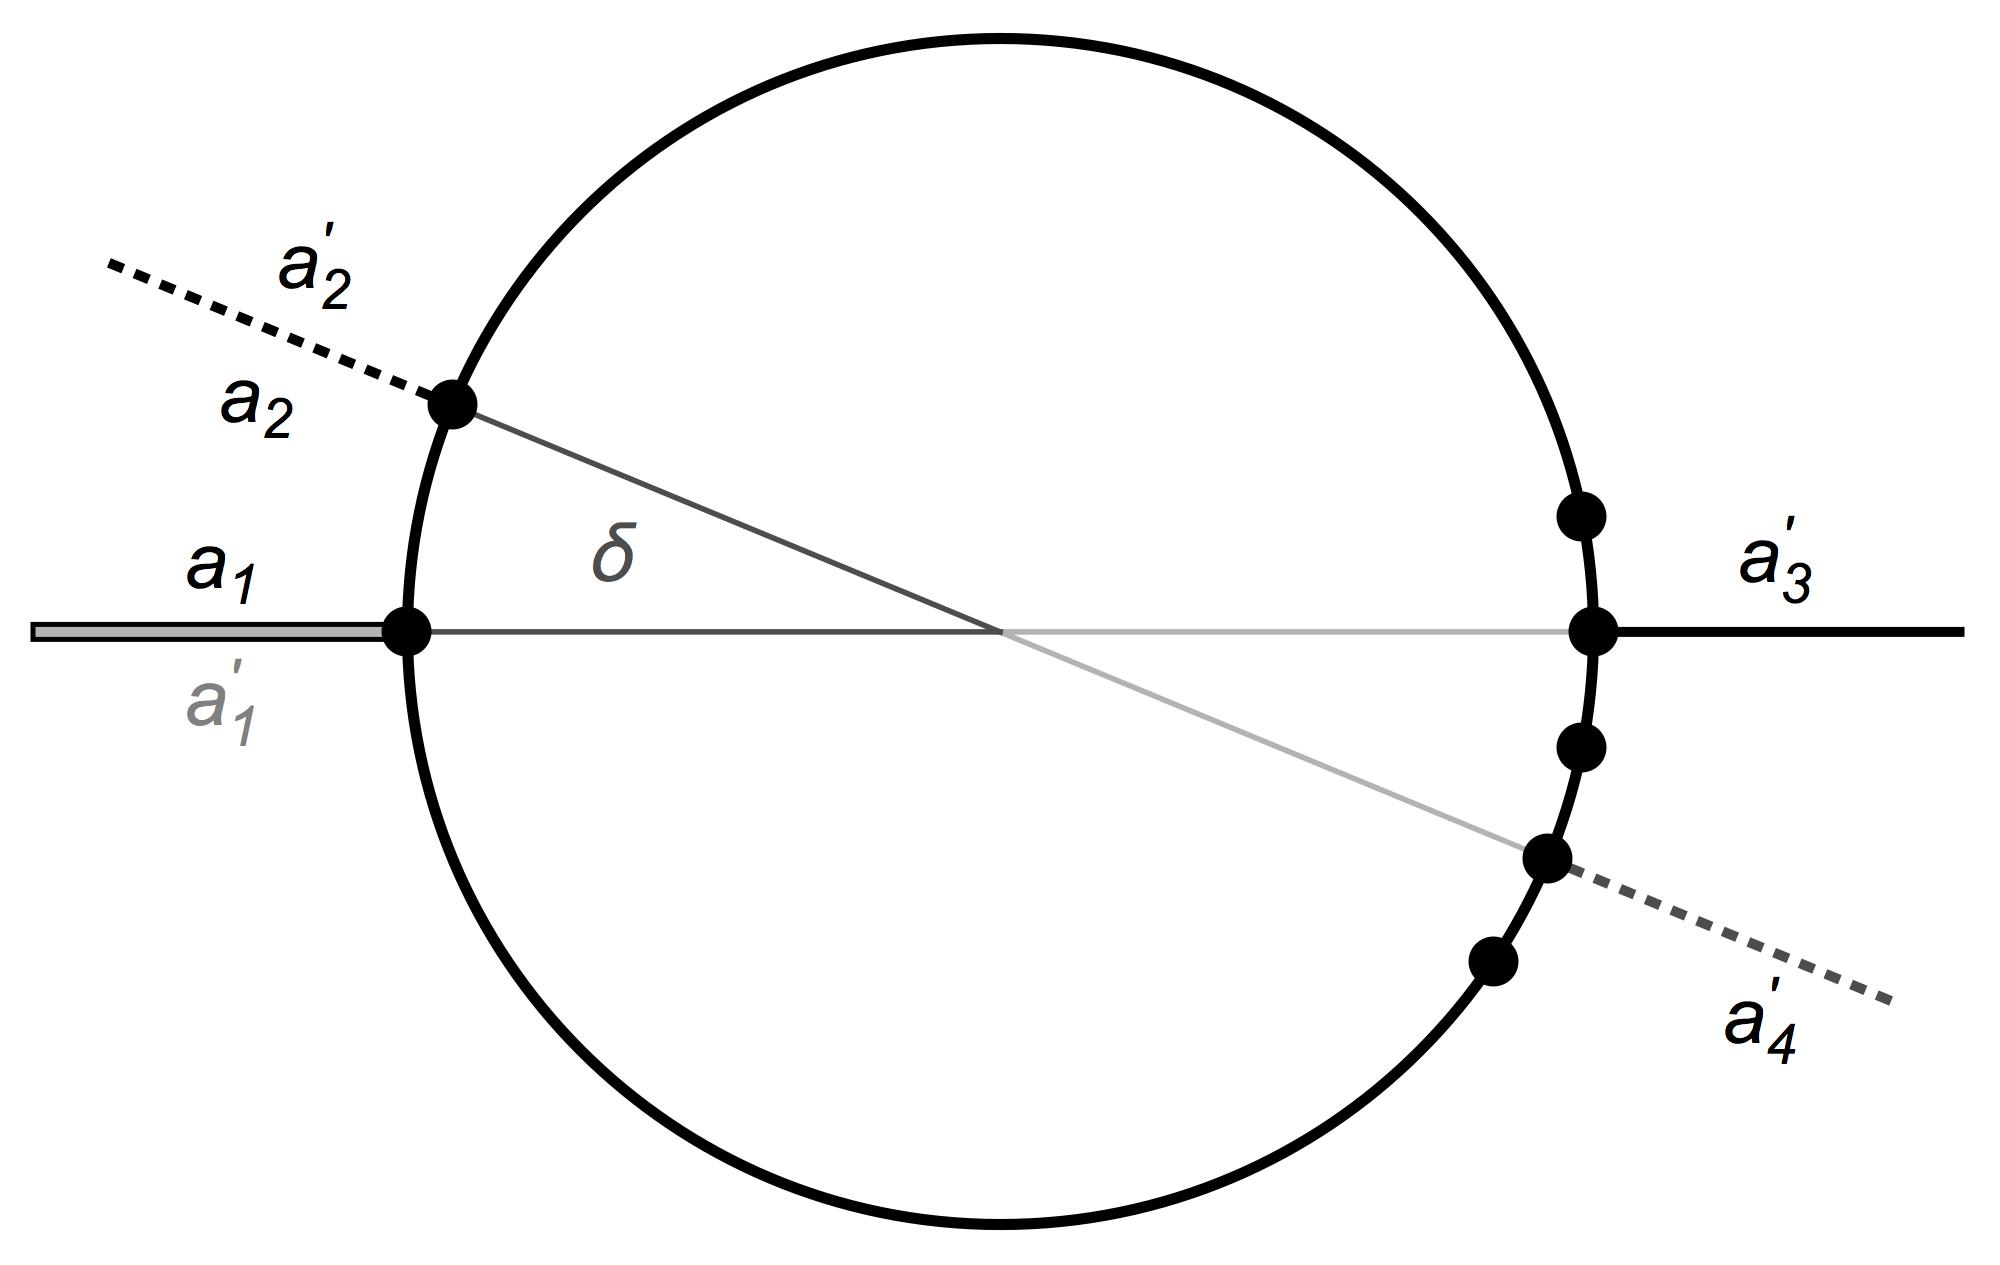
\includegraphics[width=20.0pc]{fig7.jpg}
\caption{
\small{
Multiple sources, array of drains. Two sources with amplitudes $a_1$ and $a_2$ are facing an array of drains as in the experiment \cite{Ma}. At resonance, only the aligned drains transmit with amplitudes $a_3'$ and $a_4'$. Radiation may also be reflected back to the sources with amplitudes $a_1'$ and $a_2'$.
}
\label{array}}
\end{center}
\end{figure}
%%%

Imagine now several sources are observed with an array of detectors (Fig.~\ref{array}). Suppose, for example, two sources are placed an angle $\delta$ away on the virtual sphere and are observed with a detector array, similar to the questionable part of the microwave experiments \cite{Ma}. There $\nu=9.984$, which was probably too far away from the narrow Mi\~{n}ano dip around a resonance. Consider exact resonance. According to Sec.~III~C the misaligned detectors will not fire, but will the two aligned drains transmit perfectly? Put, without loss of generality, the sources at $\theta_1=\pi$, $\theta_2=\pi+\delta$ and so the aligned drains at $\theta_3=0$, $\theta_4=\delta$, and all ports at $\phi_m=0$. Figure \ref{2o2} shows the result: the two sources are neither independently nor perfectly transmitted, unless they are farther away than about half a wavelength. Detector arrays interacting with the sources are thus not able to resolve multiple sources closer than the diffraction limit \cite{Abbe,BornWolf}.

%%%
\begin{figure}[h]
\begin{center}
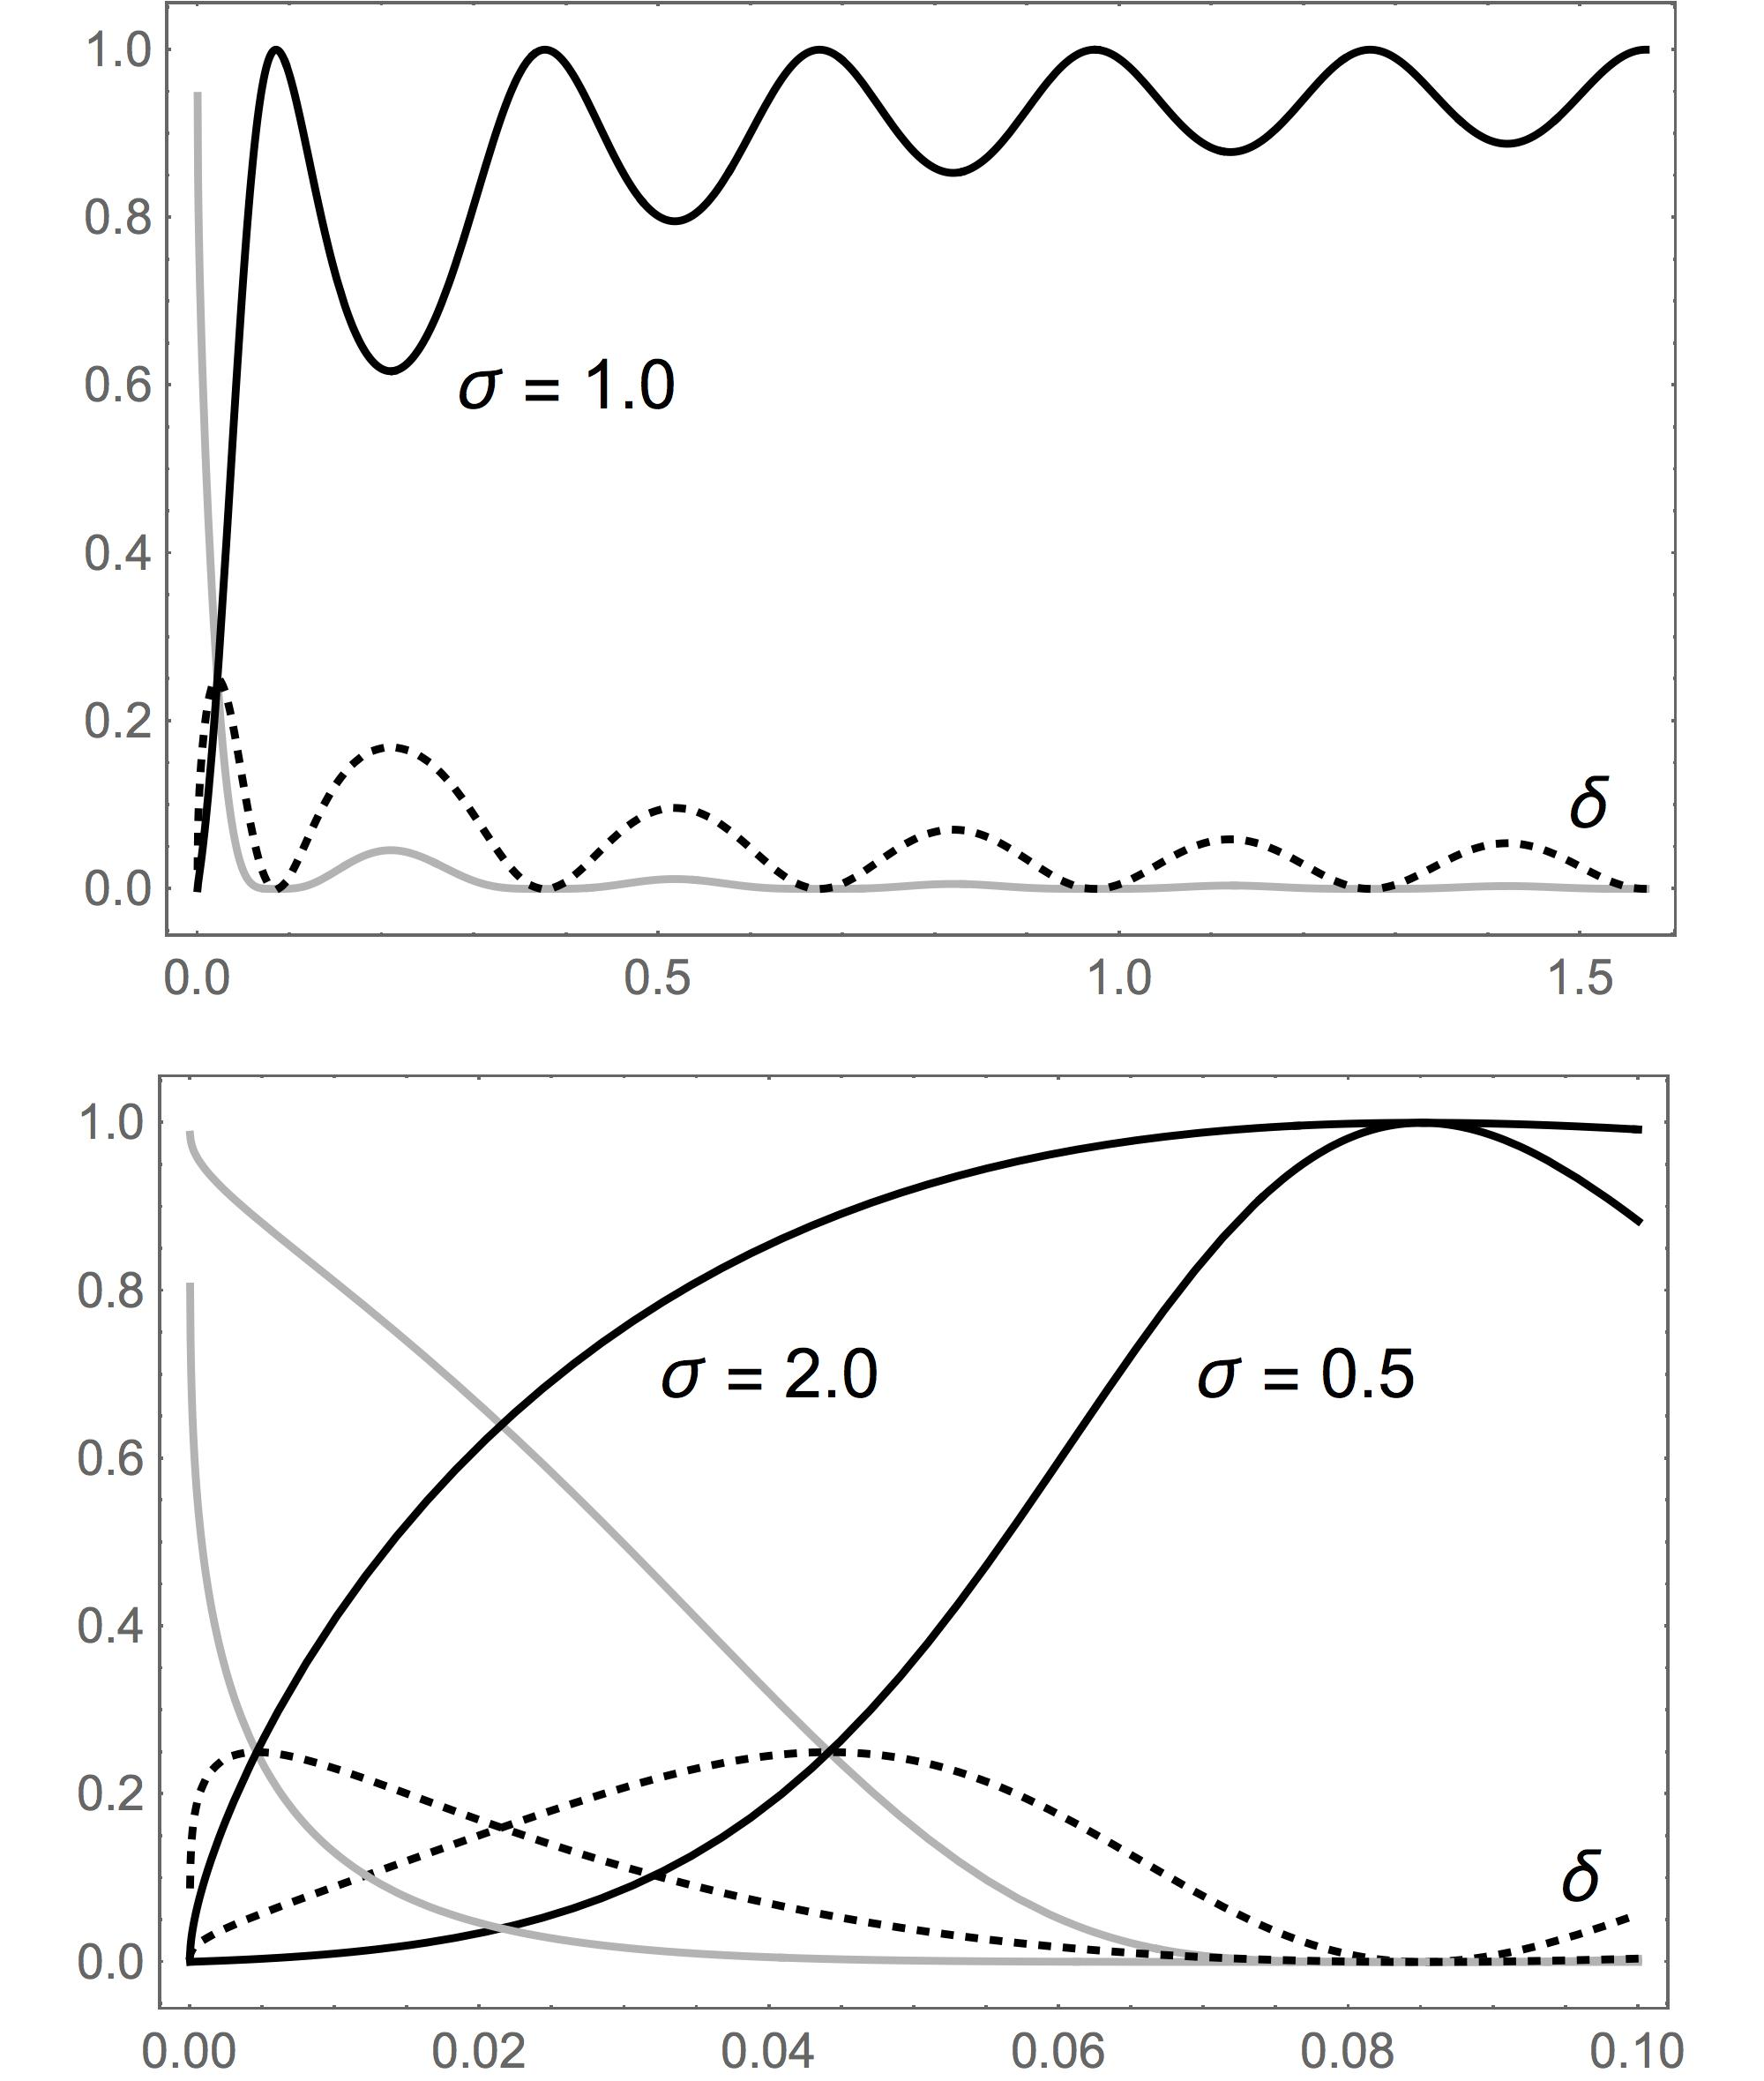
\includegraphics[width=20.0pc]{fig8.jpg}
\caption{
\small{
Two sources, two drains. Transmission of two sources separated by the angle $\delta$ to two aligned drains as a function of $\delta$ for $\nu=10$. Only one of the sources is excited ($a_1=1$, $a_2=0$). The black curves show the transmission $|a_3'|^2$, the gray curves the reflected intensity $|a_1'|^2$ and the dotted curves $|a_2'|^2=|a_4'|^2$, as indicated by the black, gray and dotted lines in Fig.~\ref{array}. Top: beyond the diffraction limit the two drains distinguish the two sources --- mostly the correct one transmits. Bottom: for a critical separation $\delta$ all the three transmission curves for fixed $\sigma$ and $\nu$ meet in a single point that depends on $\sigma$ and $\nu$. For smaller separations the transmission curves are mixed: the sources are not resolved.
}
\label{2o2}}
\end{center}
\end{figure}
%%%

\subsection{Antipodal fields}

We have analysed the imaging in Maxwell's fish eye as a scattering problem: the fields incident at the source ports and the lack of them at the drains give rise to the outgoing fields at sources and drains. We have primarily focused on a regime near resonance where we expected --- and obtained --- some properties of perfect imaging, but not all of them. Arrays of multiple sources are not perfectly imaged in detector arrays. Yet how do the fields behave? 

Consider the field $\Psi$ given by Eq.~(\ref{field}) near resonance. Assume an arbitrary number and arrangement of sources and drains. Compare the fields at one position $z$ with the field at the position that corresponds to the antipodal point on the unit sphere. The antipodes to $(X,Y,Z)$ reside at $-(X,Y,Z)$. We see from the stereographic projection of Eq.~(\ref{stereo}) that the antipodal point to $z$ is $-1/z^*$. We get from Eq.~(\ref{zeta}) that $\zeta_m$ is replaced by $-\zeta_m$ for the antipodal field. As $P_\nu(-\zeta)=(-1)^\nu P_\nu(\zeta)$ for $\nu\in\mathbb{N}$ we obtain from Eqs.~(\ref{field}) and (\ref{green}):
%%%%%%
\begin{equation}
\Psi(-1/z^*) = (-1)^\nu \Psi(z) \,.
\end{equation}
%%%%%%
The fields at $z$ and $-1/z^*$ are thus identical copies of each other, apart from the propagation factor $(-1)^\nu$. The field is antipodally symmetric --- without any symmetries in the arrangement of the sources and drains (Fig.~\ref{title} gives an example). The fields may exhibit subwavelength features, for example superoscillations \cite{Super} due to a suitable configuration of sources and drains, and yet the fields are perfect copies of each other. A negatively--refractive lens \cite{Pendry} does the same \cite{GREE}: it copies the field \cite{Dover}. Perfect imaging with positive refraction thus mimics the imaging with negative refraction. Note, however, that only the fields are copied, not the sources, and the copies are not recorded in the drains. So this feature, although interesting, is probably of rather limited practical use.

\section{Conclusions}

Feynman \cite{Feynman,Quabis} objected to Abbe's diffraction limit \cite{Abbe,BornWolf}, arguing that as Maxwell's electromagnetism is time--reversal invariant, the radiation from a point source may very well become focused in a point drain. Absolute optical instruments \cite{BornWolf} such as Maxwell's fish eye \cite{Maxwell} can perform the time reversal and may image with perfect resolution \cite{Fish}. However, the sources and drains in previous experiments \cite{Ma,Minano} were interacting with each other --- as if Feynman's drain would act back to the source in the past. Different ways of detection might circumvent this feature. The mutual interaction of sources and drains does ruin some of the promising features of perfect imaging --- arrays of sources are not necessarily resolved with arrays of detectors, but it also opens interesting new prospects in scanning near fields from far--field distances. In addition to potential practical applications, the fundamental physics of perfect imaging with interacting sources and drains illustrates how counter--intuitive wave propagation can be. Who would have thought that so much physics is hidden in Maxwell's innocent--looking fish eye?

We thank
Itay Griniasty,
Alex Kogan,
and
Tom\'{a}s Tyc
for illuminating discussions. 
Our paper was supported by QUEST from the UK Engineering and Physical Sciences Research Council, the European Research Council, the Israel Science Foundation, and a research grant from Mr. and Mrs. Louis Rosenmayer and from Mr. and Mrs. James Nathan.

%%%%%%%%%%%%%%%%%%%%%%%%%%%%%%%%%%%%

\begin{thebibliography}{99}

\bibitem{Abbe} 
E. Abbe, 
{\it Arch. Mikrosk. Anat.} {\bf 9}, 413 (1873).

\bibitem{BornWolf}
M. Born and E. Wolf,
{\it Principles of Optics}
(Cambridge University Press, Cambridge, 1999).

\bibitem{RMP}
See e.g. 
E. H. K. Stelzer, Nature {\bf 417}, 806 (2002)
about the experiment by
M. Dyba and S. W. Hell, 
Phys. Rev. Lett. {\bf 88}, 163901 (2002)
based on 
S. W. Hell and J. Wichmann, Opt. Lett. {\bf 19}, 780 (1994).

\bibitem{History}
See e.g. D. Gabor, 
Nature {\bf 161}, 777 (1948);
G. Toraldo di Francia, 
Nuovo Cimento {\bf 9}, 1943 (1952);
J. L. Harris, 
J. Opt. Soc. Am.  {\bf 54}, 931 (1964).

\bibitem{Pendry}
J. B. Pendry, 
Phys. Rev. Lett. {\bf 85}, 3966 (2000).

\bibitem{Perfectdebate}
J. R. Minkel, 
Phys. Rev. Focus {\bf 9}, 23 (2002) and references therein.

\bibitem{Fish}
U. Leonhardt, 
New J. Phys. {\bf 11}, 093040 (2009).

\bibitem{Fish3D}
U. Leonhardt and T. G. Philbin, 
Phys. Rev. A {\bf 81}, 011804 (2010); {\bf 84}, 049902 (2011).

\bibitem{Maxwell}
J. C. Maxwell,
Cambridge and Dublin Math. J. {\bf 8}, 188 (1854). 

\bibitem{Synge}
J. L. Synge, 
Trans. Amer. Math. Soc. {\bf 44}, 32 (1938).

\bibitem{TycZhang}
T. Tyc and X. Zhang, 
Nature {\bf 480}, 42 (2011).

\bibitem{Blaikie1}
R. J. Blaikie,
New J. Phys. {\bf 12}, 058001 (2010).

\bibitem{Leo1}
U. Leonhardt, 
New J. Phys. {\bf 12}, 058002 (2010).

\bibitem{Merlin1}
R. Merlin, 
Phys. Rev. A {\bf 82}, 057801 (2010).

\bibitem{LPre}
U. Leonhardt and T. G. Philbin, 
Phys. Rev. A {\bf 82}, 057802 (2010).

\bibitem{Sailing1}
F. Sun and S. He, 
PIER {\bf 108}, 307 (2010).

\bibitem{Sailing2}
F. Sun, X. C. Ge, and S. He, 
PIER {\bf 110}, 313 (2010).

\bibitem{Kinsler1}
P. Kinsler, 
Phys. Rev. A {\bf 82}, 055804 (2010).

\bibitem{LeoSahar}
U. Leonhardt and S. Sahebdivan,
J. Opt. {\bf 13}, 024016 (2011).

\bibitem{Merlin2}
R. Merlin,
J. Opt. {\bf 13}, 024017 (2011).

\bibitem{Kinsler2}
P. Kinsler and A. Favaro,
New J. Phys. {\bf 13}, 028001 (2011).

\bibitem{Leo2}
U. Leonhardt, 
New J. Phys. {\bf 13}, 028002 (2011).

\bibitem{Blaikie2}
R. J. Blaikie,
New J. Phys. {\bf 13}, 125006 (2011).

\bibitem{MinanoSim}
J. C. Mi\~{n}ano, R. Marqu\'{e}s, J. C. Gonz\'{a}lez, P. Ben�tez, V. Delgado, D. Grabovi\v{c}ki\v{c}, and M. Fre,
New J. Phys. {\bf 13}, 125009 (2011).

\bibitem{Hao}
O. Quevedo-Teruel, R. C. Mitchell-Thomas, and Y. Hao, 
Phys. Rev. A {\bf 86}, 053817 (2012).

\bibitem{Pazynin}
L. A. Pazynin and G. O. Kryvchikova, 
PIER {\bf 131}, 425 (2012).

\bibitem{TycDanner}
T. Tyc and A. Danner, 
New J. Phys {\bf 16}, 063001 (2014).

\bibitem{Sailing3}
S. He, F. Sun, S. Guo, S. Zhong, L. Lan, W. Jiang, Y. G. Ma, and T. Wu,
PIER {\bf 152}, 1 (2015).

\bibitem{1D}
U. Leonhardt, S. Sahebdivan, A. Kogan, and T. Tyc,
New J. Phys. {\bf 17}, 053007 (2015).

\bibitem{Minano}
J. C. Mi\~{n}ano, J. S\'{a}nchez-Dehesa, J. C. Gonz\'{a}lez, P. Ben�tez, D. Grabovi\v{c}ki\v{c}, J. Carbonell, and H Ahmadpanahi,
New J. Phys. {\bf 16}, 033015 (2014).

\bibitem{Nieto}
M. Nieto-Vesperinas, 
J. Opt. Soc. Am. A  {\bf 21}, 491 (2004).

\bibitem{NietoBook}
M. Nieto-Vesperinas,
{\it Scattering and Diffraction in Physical Optics}
(World Scientific, Singapore, 2007).

\bibitem{Feynman}
R. P. Feynman, R. P. Leighton, and M. Sands,
{\it The Feynman Lectures on Physics}, Vol.\ II (Addison-Wesley, San Francisco, 2006).

\bibitem{Quabis}
S. Quabis, R. Dorn, M. Eberler, O. Gl\"{o}ckl and G. Leuchs,
Opt. Commun. {\bf 179}, 1 (2000).

\bibitem{Carminati}
See also 
R. Carminati, J. J. S\'{a}enz, J. J. Greffet, and M. Nieto-Vesperinas
Phys. Rev. A {\bf 62}, 012712 (2000).

\bibitem{deRosny}
J. de Rosny and M. Fink, 
Phys. Rev. Lett. {\bf 89}, 124301 (2002).

\bibitem{Ma}
Y. G. Ma, S. Sahebdivan, C. K. Ong, T. Tyc, and U. Leonhardt, 
New. J. Phys. {\bf 13}, 033016 (2011); {\bf 14}, 025001 (2012).

\bibitem{EoC}
U. Leonhardt, S. Sahebdivan and T. Tyc, 
Expression of Concern  (unpublished).
These authors were not aware of the data manipulation committed at the time the papers \cite{Ma} were published, but became suspicious and alerted New. J. Phys. on 19 August 2014.

\bibitem{Gonzales}
J. C. Gonz\'{a}lez, P. Ben�tez, and J. C. Mi\~{n}ano, 
New J. Phys. {\bf 13}, 023038 (2011);
J. C. Gonz\'{a}lez, D. Grabovi\v{c}ki\v{c}, P. Ben�tez, and J. C. Mi\~{n}ano, 
{\it ibid.} {\bf 14}, 083033 (2012).

\bibitem{Xu}
L. Xu and H. Chen, 
Europhys. Lett. {\bf 100}, 34001 (2012).

\bibitem{MaOng}
Y. Ma, T. Wu, and C.K. Ong,
J. Opt. {\bf 15}, 125705 (2013).

\bibitem{LL2}
L. D. Landau and E. M. Lifshitz,
{\it The Classical Theory of Fields}
(Pergamon, Oxford, 1975).

\bibitem{Dover}
U. Leonhardt and T. G. Philbin, 
{\it Geometry and Light: The Science of Invisibility}
(Dover, Mineola, 2010).

\bibitem{Erdelyi}
A. Erd\'{e}lyi, W. Magnus, F. Oberhettinger, and F. G. Tricomi,
{\it Higher Transcendental Functions}
(McGraw-Hill, New York, 1981).

\bibitem{LL3}
L. D. Landau and E. M. Lifshitz,
{\it Quantum Mechanics}
(Pergamon, Oxford, 1977).

\bibitem{Super}
M. V. Berry,
{\it Faster than Fourier}
in J. S. Anandan and J. L. Safko (eds.)
{\it Quantum Coherence and Reality; in celebration of the 60th Birthday of Yakir Aharonov} 
(World Scientific, Singapore, 1994).

\bibitem{GREE}
U. Leonhardt and T. G. Philbin, 
New J. Phys. {\bf 8}, 247 (2006).

\end{thebibliography}

%%%%%%%%%%%%%%%%%%%%%%%%%%%%%%%%%%%%%%%%%%%%%%%%%%%%%%%%%%%
\end{document}



